\documentclass{scrartcl}
\usepackage[utf8]{inputenc}
\usepackage{hyperref}
\usepackage{url}
\usepackage[numbers]{natbib}
\usepackage{graphicx}
\usepackage{float}
\usepackage{array}
\usepackage{booktabs}
\usepackage{tikz}
\usetikzlibrary{positioning, backgrounds, arrows.meta}
\usepackage{cleveref} % this must be the last package to be loaded

\newcommand{\emailaddr}[1]{\href{mailto:#1}{\texttt{#1}}}

\title{\LARGE
    Distributed Lupus in Fabula\\
    A Replicated Real-Time Multiplayer Game Platform
}
\subtitle{Final Report for the Distributed Systems Course --- A.Y. 2025/2026}

\author{
    Leonardo Vorabbi \\ \emailaddr{leonardo.vorabbi@studio.unibo.it}
    \and
    Jacopo Bonifazi \\ \emailaddr{jacopo.bonifazi@studio.unibo.it}
    \and
    Alexandru Nicolescu \\ \emailaddr{alexandru.nicolescu@studio.unibo.it}
}

\date{\today}

\begin{document}

\maketitle

\begin{abstract}
      Distributed Lupus in Fabula is a real-time multiplayer web application that brings the classic social deduction game Lupus in Fabula online, allowing groups of players to create or join a game lobby from any browser and play a full match together over the internet.
      The system is composed of a Vue 3 single-page frontend and a FastAPI/Socket.IO backend, communicating via REST for stateless operations and via WebSocket for real-time, low-latency interactions such as votes, phase transitions, and private role actions. Game and lobby state is kept in Redis rather than a traditional database, acting both as a shared source of truth across backend replicas and as a Pub/Sub broker that lets events generated on one instance reach clients connected to any other instance.
      This design allows the backend to run as multiple concurrent, interchangeable replicas behind a reverse proxy, supporting many simultaneous matches while keeping every player's view of the game synchronized in real time.
\end{abstract}

\section*{Disclaimer}

During the preparation of this work, the authors used LLM-based tools (Claude) to refine syntax, correct linguistic errors, core review and the refinement of infrastructure configuration files.
After using this tool, the authors reviewed and edited the content as needed and take full responsibility for the content of the final report/artifact.

\section{Concept}\label{Concept}

\subsection{Type of Product}\label{type-of-product}

The project is a web application, specifically a real-time multiplayer game
inspired by the traditional social deduction game \emph{Lupus in Fabula}. It
is a full-stack distributed system composed of:

\begin{itemize}
      \item a \textbf{frontend}: a Vue~3 Single Page Application (SPA), accessible
            via browser, with no installation required;
      \item a \textbf{backend}: a set of stateless, horizontally replicated web
            services built with FastAPI and Socket.IO, responsible for game logic,
            session management, and real-time event propagation;
      \item a \textbf{shared data layer}: Redis, used both as a low-latency state
            store and as a Pub/Sub message broker connecting the backend replicas.
\end{itemize}

These are complemented by an infrastructure layer (reverse proxy / ingress,
monitoring stack) that is part of the deliverable (\cref{infrastructure}). The
whole system is designed to be deployed as a multi-container distributed
application rather than as a single monolithic server.

\subsection{Use Case Description}\label{use-case}

\paragraph{What the software does.}
The application lets a group of 5 or more players create or join a virtual
``lobby'', wait until everyone is ready, and then play a phase-based game of
hidden roles and social deduction. Players are secretly split into two
factions: \emph{wolves}, who eliminate one villager per night, and
\emph{villagers} (possibly including a \emph{seer}, who can privately inspect
one player's faction each night), who try to identify and lynch the wolves
through a public vote. Once a match starts, the game state moves automatically
through a fixed sequence of phases driven by server-side timers:
\[
      \textbf{LOBBY} \rightarrow \textbf{NIGHT} \rightarrow \textbf{DAY}
      \rightarrow \textbf{VOTING} \rightarrow \cdots \rightarrow \textbf{ENDED}.
\]
During NIGHT, players with special roles perform hidden actions that the server
resolves before the next day begins; during DAY/VOTING, players discuss and
vote to eliminate a suspect. The match ends automatically once a win condition
is met, and the server is authoritative throughout: it assigns hidden roles,
collects votes and night actions, computes eliminations, and detects the
winner.

\paragraph{Where the users are.}
Players are geographically dispersed (or at least not necessarily co-located):
each player connects independently from their own browser, over the public
Internet, to a shared game session identified by a room/lobby code. The service
itself runs in a datacenter (a container orchestration cluster).

\paragraph{When and how frequently they interact.}
Interaction is continuous and real-time for the whole duration of a match
(several minutes to tens of minutes), not just at fixed request/response
intervals. Players must react within phase time limits (voting windows,
night-action windows), so the system needs low-latency, event-driven
communication rather than periodic polling.

\paragraph{How they interact.}
All interaction happens through a web browser via the Vue SPA. The frontend
communicates with the backend in two complementary ways:
\begin{itemize}
      \item \textbf{REST} calls for stateless operations such as creating a lobby,
            joining a lobby, or fetching the current game state;
      \item \textbf{WebSocket} (Socket.IO) for real-time, bidirectional events:
            votes, phase changes, chat, private role actions, disconnect/reconnect
            notifications.
\end{itemize}

\paragraph{Does the system store user data? Which, and where?}
The system does not use a persistent relational database for user accounts,
since there is no long-term profile storage. Instead it relies on Redis as a
shared, TTL-based store for all session-scoped game data:
\begin{itemize}
      \item room/lobby state and configuration;
      \item the list of connected players and their ready status;
      \item assigned roles (Wolf, Seer, Villager);
      \item votes cast during the DAY/VOTING phase and private night actions;
      \item phase timers and current phase;
      \item host identity.
\end{itemize}
Clients are never trusted with authoritative data (a client that knew the role
assignments could cheat), and state expires automatically (TTL) hours after
the last update, so no long-term personal data is persisted. On the client
side, the browser retains a minimal amount of session data in local storage,
purely to support reconnection and continuity across page reloads or brief
disconnects.

\begin{figure}
      \centering
      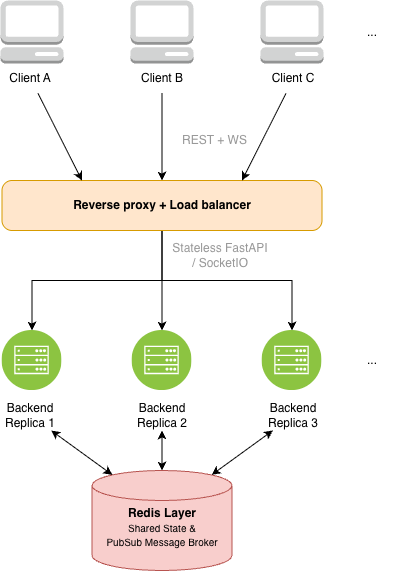
\includegraphics[width=0.55\textwidth]{figures/system_architecture_overview.png}
      \caption{High-level architecture: clients connect through a reverse proxy to
            stateless backend replicas, which share game state and propagate events
            through Redis.}
      \label{fig:architecture}
\end{figure}

\paragraph{Roles.}
The system distinguishes several actor roles at different levels:
\begin{itemize}
      \item \emph{Application-level roles}: \textbf{Villager}, \textbf{Wolf},
            \textbf{Seer}, each with different permitted actions and visibility (e.g.\
            wolves share a private night chat and see each other's votes; the seer can
            inspect one player per night);
      \item \emph{Session-level roles}: the \textbf{host}, who configures the
            match, can remove players from the lobby, starts the game, and restarts it
            once ended, versus \textbf{regular players}, who can only join, ready up,
            vote, and act according to their assigned role; the host role migrates
            automatically if the current host disconnects;
      \item \emph{System role}: the backend itself acts as an autonomous
            \textbf{orchestrator}. It owns the authoritative game state, advances phases
            via timers, resolves votes and night actions, and enforces which actions are
            legal at any given moment.
\end{itemize}

\subsection{Why Distribution Is Needed}\label{why-distribution}

Distribution in this project is not motivated by geographic proximity to users,
but primarily by scalability, real-time synchronization, and fault tolerance:

\begin{itemize}
      \item \textbf{Horizontal scalability / resource sharing.} The backend is
            designed to run as multiple stateless replicas behind a reverse proxy, so
            that many concurrent lobbies and matches can be served in parallel without a
            single process becoming a bottleneck. Because game state lives in Redis
            rather than in each process's memory, any replica can handle requests for any
            room, allowing the system to scale out simply by adding more backend
            instances.

      \item \textbf{Shared state across replicas.} Since each backend instance is
            stateless with respect to game data, Redis acts as the single source of truth
            for lobby/game state. This is what makes horizontal scaling actually work: a
            player's WebSocket connection can be handled by one replica while another
            replica processes a REST call for the same match, and both see a consistent
            view of the state.

      \item \textbf{Cross-replica real-time propagation.} Because clients belonging
            to the same room can be connected to different backend replicas, a simple
            in-process event emitter is not sufficient. The system uses Redis Pub/Sub to
            broadcast game events (vote updates, phase transitions, chat messages, etc.)
            across all replicas, ensuring that every client in a room receives updates
            regardless of which instance generated them or which instance is handling
            their socket.

      \item \textbf{Fault tolerance and continuity.} The backend includes explicit
            mechanisms for reconnecting to Redis, retrying failed operations,
            sweeping/recovering timers, and reconciling state after temporary
            inconsistencies (anti-entropy). This matters because a real-time game cannot
            simply crash or stall if a single backend replica fails, a Redis connection
            drops momentarily, or a player's browser disconnects and reconnects
            mid-match. The match state and timers must survive these events.

      \item \textbf{Reduced dependency on a single instance.} Because the game
            state is decoupled from any specific process, a backend replica can be
            restarted, replaced, or scaled down/up without necessarily terminating
            ongoing matches, and a reconnecting player can resume their session against a
            different replica than the one they were originally connected to.
\end{itemize}

In summary, this system is distributed primarily to support many concurrent
matches, keep real-time state synchronized across independent backend replicas,
and remain resilient to instance failures and client disconnections.

\section{Requirements Elicitation and Analysis}\label{requirements}

This section specifies \emph{what} the system must do, independently of the
implementation strategies later adopted. Requirements are grouped into
functional, non-functional, and implementation requirements, each with a unique
identifier and an associated acceptance criterion (AC) used during validation.

\subsection{Glossary}\label{glossary}

\begin{description}
      \item[Room (or lobby)] An independent game session, identified by a
            user-chosen code, hosting one match at a time.
      \item[Host] The player who administers a room: configures the match, starts
            it, kicks players, and restarts the game once it has ended.
      \item[Phase] A stage of the game loop: \textsc{lobby}, \textsc{night},
            \textsc{day}, \textsc{voting}, \textsc{ended}.
      \item[Role] The secret game faction assigned to a player: \emph{wolf},
            \emph{seer}, or \emph{villager}.
      \item[Replica (or instance)] One of the interchangeable backend server
            processes serving client connections.
      \item[Snapshot] The complete, authoritative representation of a room's state,
            as stored server-side and sent to (re)connecting clients.
\end{description}

\subsection{Functional Requirements}\label{functional-requirements}

\begin{description}
      \item[FR1 --- Room creation and joining.] A user can create or join a room by
            choosing a nickname and a room code; the first user entering a room becomes
            its host. \emph{AC: two users entering the same code end up in the same
                  lobby; exactly one host exists, even if two users create the same room
                  simultaneously.}

      \item[FR2 --- Lobby browsing.] A user can list the currently open rooms
            (those still in \textsc{lobby} phase) with their host and player count.
            \emph{AC: a room in progress or ended does not appear in the list; an open
                  room appears regardless of which replica serves the request.}

      \item[FR3 --- Match configuration.] The host, and only the host, can
            configure the number of wolves and seers while in \textsc{lobby}.
            Configurations that break the game balance are rejected (at least 5 players,
            at least 1 wolf, at least 1 plain villager left). \emph{AC: a non-host attempt
                  or an invalid configuration is refused with an error message; a valid change
                  is visible to all lobby members.}

      \item[FR4 --- Readiness and game start.] Players declare themselves ready; the
            host can start the match only when all connected players are ready and the
            configuration is valid. \emph{AC: a start request with a non-ready player is
                  rejected; on start, every player receives their secret role.}

      \item[FR5 --- Secret role assignment.] At game start the system randomly
            assigns roles according to the configuration; each player learns \emph{only}
            their own role (wolves also learn their teammates). \emph{AC: no message
                  delivered to a villager's client ever contains another player's role before
                  game end.}

      \item[FR6 --- Game loop and timers.] The game alternates
            \textsc{night} $\to$ \textsc{day} $\to$ \textsc{voting} phases, each bounded
            by a server-side timer; when the timer expires the phase advances
            automatically for everyone. \emph{AC: phases advance without any client input;
                  all clients converge on the same phase and deadline.}

      \item[FR7 --- Public vote.] During \textsc{voting} every living player can
            vote a living target (or skip); votes are public, ties or skip-majority cause
            no elimination; the most-voted player is eliminated and their role revealed.
            \emph{AC: dead or disconnected players cannot vote; the tally matches the
                  recorded votes even when voters are connected to different replicas.}

      \item[FR8 --- Night actions.] During \textsc{night}, wolves privately agree on
            a victim (seeing each other's votes), and the seer privately inspects one
            player's faction. \emph{AC: night choices are never visible to other players;
                  the seer's result is delivered only to the seer, even if connected to a
                  different replica than the one computing it.}

      \item[FR9 --- Win detection.] The system detects the end of the game as soon
            as a faction wins (no wolves left, or wolves $\geq$ non-wolves) --- including
            when the decisive event is a player abandoning the match --- and reveals all
            roles. \emph{AC: the ended screen shows winner and roles to every player; no
                  further game action is accepted.}

      \item[FR10 --- Chat.] Players in a room can exchange real-time chat messages
            over restricted-visibility channels (a global channel during the day, a
            wolves-only channel at night, and a dead-players channel); system
            announcements (e.g.\ a player fleeing mid-game) appear in the same feed.
            \emph{AC: a message on a restricted channel is rendered only by the clients
                  entitled to see it, and a message sent by a player on replica $A$ reaches
                  entitled players on replica $B$.}

      \item[FR11 --- Reconnection.] A player who loses the connection mid-game can
            rejoin the same room with the same nickname and receive the current
            authoritative state (including their role). \emph{AC: after a page reload
                  during a match, the player sees the current phase, timer, and their own role,
                  even when reconnected to a different replica.}

      \item[FR12 --- Host migration.] If the host disconnects, another connected
            player is automatically promoted host. \emph{AC: the lobby never remains
                  without a host while at least one player is connected.}

      \item[FR13 --- Room administration.] The host can kick a player from the
            lobby, and can restart a finished game bringing everyone back to the lobby
            (with roles, votes, and readiness reset, and disconnected players cleaned up).
            \emph{AC: a kicked player is removed from every registry and notified; after
                  restart, no ``ghost'' player remains and nobody is marked ready.}

      \item[FR14 --- Access control to running games.] A user who is not part of a
            match cannot join a room where a game is in progress or ended, and a nickname
            already connected to a room cannot be reused concurrently. \emph{AC: the
                  connection is refused with an explanatory message.}
\end{description}

\begin{figure}
      \centering
      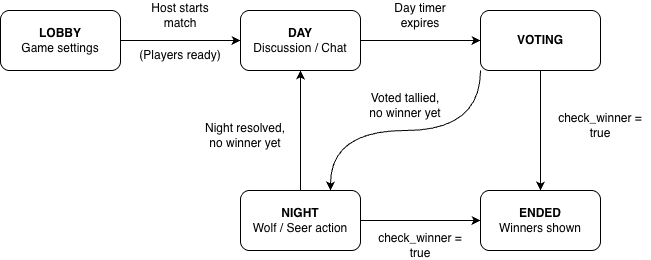
\includegraphics[width=0.9\textwidth]{figures/game_state_machine.png}
      \caption{State machine of the match phases. Transitions are driven
            automatically by server-side timers and by \texttt{check\_winner()}.}
      \label{fig:phase-state-machine}
\end{figure}

\subsection{Non-Functional Requirements}\label{non-functional-requirements}

\begin{description}
      \item[NFR1 --- Replication transparency.] Clients must not know, or care,
            which backend replica serves them: any replica must be able to serve any room,
            and two players in the same room must be able to play together while connected
            to different replicas. \emph{AC: the multi-instance test suite passes with 2+
                  replicas behind the load balancer.}

      \item[NFR2 --- Fault tolerance.] The crash of a single backend replica must
            not destroy any running match: affected clients reconnect and resume within
            seconds; matches served by other replicas must not be affected. Phase
            progression must not depend on the survival of the replica that scheduled the
            current phase timer. \emph{AC: killing one replica during a match, the game
                  reaches its natural end.}

      \item[NFR3 --- Convergence (eventual consistency).] All clients of a room must
            converge to the same authoritative game state: temporarily missed events must
            be repaired automatically within seconds, without user intervention.
            \emph{AC: a client that missed a broadcast converges to the authoritative
                  snapshot within one anti-entropy period ($\sim$10\,s).}

      \item[NFR4 --- Safety of game rules.] Game-rule invariants must hold despite
            concurrency and replication: no lost updates on shared state, at most one host
            per room, at most one phase advancement per deadline (no double eliminations).
            \emph{AC: the distributed-safety test suite passes with concurrent clients on
                  multiple replicas.}

      \item[NFR5 --- Scalability.] Capacity (concurrent connections/rooms) must grow
            by adding backend replicas, with no code changes and no single-replica
            bottleneck in the service tier; the deployment must support automatic
            horizontal scaling. \emph{AC: under load, the autoscaler increases replicas
                  and new connections are spread across them.}

      \item[NFR6 --- Soft real-time interactivity.] Game events must reach all
            players of a room with sub-second perceived latency under nominal load.
            \emph{AC: load tests report end-to-end event fan-out latencies well below
                  1\,s at the target load.}

      \item[NFR7 --- Observability.] Operators must be able to inspect the health
            and behaviour of every component (connections per replica, Pub/Sub traffic,
            error rates, resource usage) through metrics, dashboards, and alerts.
            \emph{AC: Grafana dashboards display per-replica WebSocket and Redis metrics;
                  alert rules fire on component failure.}

      \item[NFR8 --- Zero-downtime updates.] Deploying a new backend version must
            not interrupt the service. \emph{AC: a rolling update completes with no failed
                  health checks and no window with zero ready replicas.}

      \item[NFR9 --- Usability.] The interface must let a non-technical user join
            and play a match without understanding the system's internal details.
            \emph{AC: a user can complete lobby creation/joining, the lobby phase, and the
                  match using only a browser and a room code.}
\end{description}

\subsection{Implementation Requirements}\label{implementation-requirements}

By design (\cref{design}) the system needs an asynchronous, WebSocket-capable
service runtime, a shared low-latency store with publish/subscribe capabilities,
and reproducible containerised deployment. The concrete constraints below
descend from those needs plus course/administrative context:

\begin{description}
      \item[IR1] The system shall be containerised and runnable both with Docker
            Compose (local, single machine) and on Kubernetes (cluster), since deployment
            automation and orchestration are learning goals of the project. \emph{AC: both
                  \texttt{docker compose up} and the provided Kubernetes manifests bring up the
                  full platform.}

      \item[IR2] The backend shall expose Prometheus-compatible metrics, as
            Prometheus + Grafana is the de-facto standard open-source monitoring stack and
            fits the zero-budget constraint. \emph{AC: \texttt{/metrics} is scraped
                  successfully by the provided Prometheus configuration and visualised in
                  Grafana.}

      \item[IR3] Only free / open-source components shall be used (no managed cloud
            services), for economic reasons and local reproducibility on student machines.
            \emph{AC: the whole platform runs on a laptop via minikube.}
\end{description}

Programming languages and frameworks (Python/FastAPI, Vue.js, Redis) were
\emph{not} imposed a priori; they emerge as consequences of the design and are
motivated in \cref{implementation}.

\subsection{Relevant Distributed System Features}\label{ds-features}

We assess which classic distributed-system
concerns~\cite{tanenbaum2017distributed} are relevant for this project, and to
what extent.

\begin{description}
      \item[Transparency --- central.] \emph{Replication} and \emph{access}
            transparency are the core of the project: users must perceive a single logical
            game server, while connections are actually served by interchangeable replicas
            (NFR1). \emph{Failure} transparency is pursued for server-side faults (a
            replica crash appears as a brief reconnection, not a lost match --- NFR2).
            \emph{Location} transparency is provided by naming services and virtual hosts
            (clients address \texttt{game.local}, never a specific pod). Migration,
            relocation, and persistence transparency are not relevant: components do not
            move at runtime and no long-term persistence is exposed to users.

      \item[Fault tolerance / dependability --- central.] The service tier must
            tolerate crash failures (fail-stop) of any single replica, and temporary
            unavailability of the message bus. Uninterrupted service is required at match
            granularity: losing a running match is the failure to avoid. Recovery must be
            fast (seconds), since matches are paced by timers. Byzantine behaviour of
            \emph{servers} is out of scope (all replicas are trusted, deployed from the
            same image); malicious \emph{clients} are considered only at the game-rule
            level (the server is authoritative, FR5/FR14). Durability beyond a match is
            explicitly \emph{not} required: game state is ephemeral, which licenses an
            in-memory store with TTL-based garbage collection rather than a durable
            database.

      \item[Scalability --- central.] The system must scale \emph{out} with the
            number of concurrent players and rooms (NFR5). Rooms are independent, so the
            workload partitions naturally; the stateless service tier scales horizontally
            while the shared store stays small (per-room state is a few KB) and is not the
            bottleneck at the target scale. Geographic (multi-datacenter) scalability is
            out of scope.

      \item[Security / trust --- limited relevance.] No sensitive or personal data
            is stored (nicknames only), so confidentiality and GDPR-style concerns are
            minimal. What matters is \emph{authorization} at the application level:
            host-only administrative actions (FR3, FR13) and role-based information hiding
            during a match (FR5, FR8) --- trust is placed in the server, never in clients.
            Strong authentication is deliberately absent (casual, friction-free party
            game); the perimeter is protected by rate limiting and security headers at the
            proxy. TLS is prepared for but not enabled in the local deployments.

      \item[Resource sharing --- central.] All replicas share the authoritative
            state store and the inter-replica event bus; all rooms share the replica pool.
            This is precisely what requires the coordination and synchronisation
            mechanisms (atomic updates, distributed locks) described in
            \cref{data-and-consistency-issues}.

      \item[Performance / concurrency --- central.] The workload is massively
            concurrent (many rooms, many sockets) but computationally light: the challenge
            is efficient I/O multiplexing and fan-out, not CPU. This drives the choice of
            an asynchronous, event-loop-based runtime and of connection-aware load
            balancing; per-message bandwidth is negligible (small JSON events).
\end{description}

Conversely, some concerns are deliberately \emph{non-central}: geographical
distribution (no geo-aware routing or replication is required), heterogeneity
beyond the standard web stack (all components speak HTTP/WebSocket/JSON, with no
integration of complex third-party systems), and a strong security model (no
critical personal data or financial transactions are handled).

\section{Design}\label{design}

This chapter explains the strategies used to meet the requirements identified in
the analysis. The design is described in technology-neutral terms wherever
possible; concrete technology bindings are deferred to \cref{implementation}.

\subsection{Architecture}\label{architecture}

The system combines two classic architectural styles over a client/server
organisation.

\paragraph{Layered (three-tier) backbone.}
At the coarse grain the system is a \emph{three-tier layered} architecture: a
\textbf{presentation tier} (the SPA running in each player's browser), an
\textbf{application tier} (a pool of identical, \emph{stateless} game-server
replicas behind a load-balancing proxy), and a \textbf{data tier} (a shared
in-memory store holding all authoritative state). The backend does not treat its
in-memory representation as authoritative; it reconstructs domain state from
Redis on demand and uses Pub/Sub purely as a notification mechanism, never as a
source of truth. Layering gives separation of concerns and lets each tier scale
independently: the application tier scales horizontally precisely \emph{because}
it is stateless --- ``stateless servers + stateful store'' is the standard recipe
for service redundancy~\cite{kleppmann2017designing}, and it directly serves
NFR1/NFR5.

\paragraph{Event-based core.}
Within a match interaction is not request/response: the dominant flow is
\emph{events} (a vote was cast, a phase changed, a player was eliminated) that
must be \emph{pushed} to all interested parties with low latency (NFR6). The
architecture is therefore \emph{event-based} at two levels:
\begin{itemize}
      \item between server and clients, each room acts as a topic: clients subscribe
            by joining the room, and the server pushes domain events to all of its members
            over persistent connections;
      \item between server replicas, a \emph{publish/subscribe event bus} (one
            logical channel per room, hosted by the data tier) propagates every event to
            the other replicas, which relay it to their locally connected clients.
\end{itemize}
The publish/subscribe connector is what makes replication transparent (NFR1):
replicas are \emph{referentially and spatially uncoupled} --- they never address
each other, do not know how many peers exist, and need no membership protocol;
the set of replicas can change at any time (autoscaler, crash, rolling update)
without reconfiguration~\cite{tanenbaum2017distributed}.

\paragraph{Client-side layering.}
The frontend is itself a Single-Page Application organised in three internal
layers, so that the client stays event-driven and \emph{stateless with respect
      to game logic}: \textbf{views} present state and collect input but never touch
the network; \textbf{stores} hold the reactive client state, register listeners
for server events, and expose the actions that emit commands; a single
\textbf{communication layer} (a Socket.IO wrapper) is the only component that
touches the network. Because the client holds no authoritative state, it can
always be re-synchronised from the server after a fault and behaves identically
regardless of the instance it is attached to (N2/N3 of the client scope).

\paragraph{Why not alternatives.}
A single stateful game server (state in process memory, no bus) would be simpler
but violates NFR2/NFR5: a single point of failure and a vertical-scaling dead
end. Sticky sessions (pinning a whole room to one replica) would remove the need
for the bus but reintroduce the same problem at room granularity --- a replica
crash would still destroy its rooms --- and defeat connection-level load
balancing. Peer-to-peer distribution among clients was discarded because hidden
roles (FR5) demand an authoritative, trusted party that clients cannot inspect.
Finally, consensus-based state-machine replication across
replicas~\cite{schneider1990implementing} was deliberately avoided: it would
provide stronger consistency than the game needs, at the price of latency and
complexity (\cref{data-and-consistency-issues} argues that a shared atomic store
plus eventual client convergence is sufficient).

\subsection{Infrastructure}\label{infrastructure}

\paragraph{Components.}
The deployed system comprises the following components:
\begin{description}
      \item[Clients ($N$).] One browser per player, holding a single persistent
            bidirectional connection plus occasional REST calls.
      \item[Reverse proxy / load balancer (1).] The single entry point. It routes by
            path --- real-time traffic and the REST API to the backend pool, everything
            else to the frontend --- terminates and upgrades WebSocket connections, applies
            per-IP rate limiting (\cref{security}), and balances \emph{new connections}
            across backend replicas round-robin. In the orchestrated deployment this role
            is played by the cluster's ingress controller.
      \item[Frontend static server (1--2).] Serves the SPA assets. Trivially
            replicable since it holds no state; at page load it injects the runtime
            configuration (the backend origin) so the same image works in every
            environment.
      \item[Backend replicas (2--8).] Identical stateless game servers. Two is the
            floor (no single point of failure in the service tier, NFR2); the ceiling is
            set by the autoscaler (NFR5). Each replica has a unique \emph{instance
                  identifier} used for event deduplication, distributed-lock ownership, and
            per-replica metrics.
      \item[Shared store / message broker (1).] A single in-memory data store
            playing \emph{two} roles at once: the authoritative state database (key--value
            snapshots, hashes for player registries and vote maps) and the inter-replica
            publish/subscribe broker (one channel per room plus a global channel).
            Collapsing the two roles keeps the infrastructure minimal (IR3). The store is a
            deliberate single stateful instance --- \cref{fault-tolerance} discusses how
            its temporary unavailability is tolerated and \cref{future-works} sketches its
            high-availability evolution.
      \item[Monitoring stack (3).] A metrics scraper/time-series database (pull-based
            collection from every backend replica and from a store-metrics exporter), a
            dashboard server, and the exporter itself (NFR7, IR2). Pull-based scraping was
            preferred to push because replicas come and go (autoscaling): the scraper
            discovers targets dynamically instead of each ephemeral replica registering
            itself.
\end{description}

\begin{figure}
      \centering
      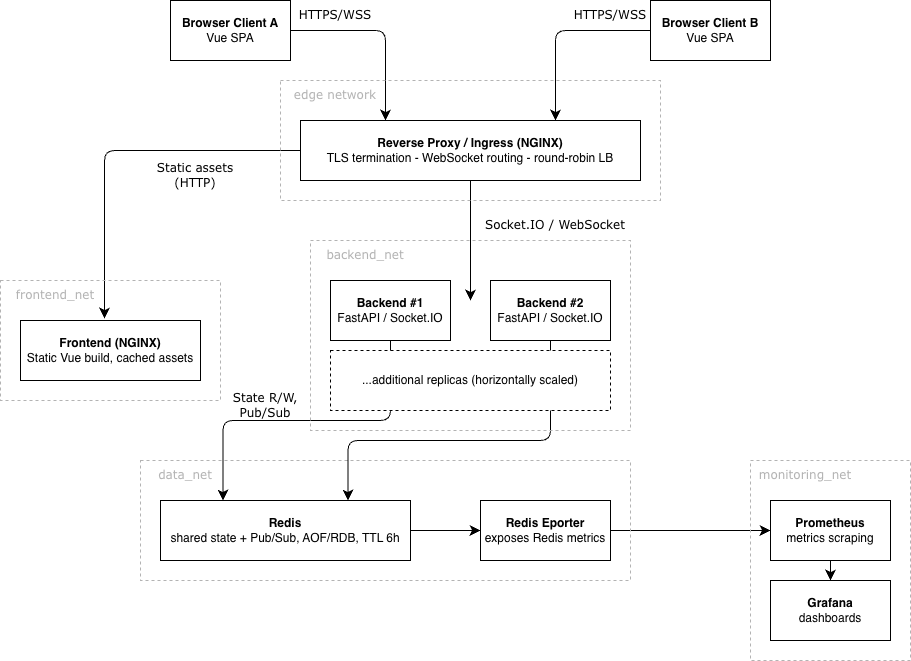
\includegraphics[width=0.85\textwidth]{figures/component_diagram.png}
      \caption{Component diagram: logical components and their dependencies ---
            browser clients, the reverse proxy / ingress, the frontend static server,
            the pool of backend replicas, the shared Redis store $+$ broker, and the
            monitoring stack.}
      \label{fig:component}
\end{figure}

\paragraph{Network placement.}
All server-side components run in the same cluster/datacenter --- distribution
here serves fault tolerance and scalability, not geo-proximity
(\cref{ds-features}). Latency-critical hops (replica $\leftrightarrow$ store) are
intra-cluster and sub-millisecond. Clients reach the cluster over the public
Internet through the single proxy entry point. Internally the network is
segmented into four bridge networks (\cref{tab:networks}): the proxy can reach
the frontend and the backend pool but \emph{not} the store; the store sits on two
networks, reachable by the backends (data path) and by the observability stack
(monitoring path). The edge tier and the store share no network at all, which
confines the blast radius of a compromised edge component. In Kubernetes the same
segmentation is reproduced through separate Services and namespaced routing, with
backend and Redis exposed only as internal \texttt{ClusterIP} services and
external traffic entering exclusively through the NGINX Ingress.

\begin{table}
      \centering
      \caption{Network membership of each component in the Docker Compose topology.
            Two components can talk at the network layer \emph{iff} they share a bridge
            network. The edge proxy shares no network with the store, which confines the
            blast radius of a compromised edge; the store is reachable on
            \texttt{data\_net} by the backends and on \texttt{monitoring\_net} by the
            observability stack.}
      \label{tab:networks}
      \begin{tabular}{lcccc}
            \toprule
                                         & \multicolumn{4}{c}{\emph{Bridge network}}                                                \\
            \cmidrule(l){2-5}
            Component
                                         & \texttt{frontend}                         & \texttt{backend} & \texttt{data}
                                         & \texttt{monitoring}                                                                      \\
            \midrule
            Reverse proxy / Ingress      & $\bullet$                                 & $\bullet$        &               &           \\
            Frontend static server       & $\bullet$                                 &                  &               &           \\
            Backend replica ($\times N$) &                                           & $\bullet$        & $\bullet$     &           \\
            Redis (store $+$ bus)        &                                           &                  & $\bullet$     & $\bullet$ \\
            Prometheus                   &                                           & $\bullet$        &               & $\bullet$ \\
            Grafana                      &                                           &                  &               & $\bullet$ \\
            redis-exporter               &                                           &                  &               & $\bullet$ \\
            \bottomrule
      \end{tabular}
\end{table}

\paragraph{Naming and discovery.}
Components find each other by \emph{name}, never by address: clients use one
virtual host (e.g.\ \texttt{game.local}) for everything --- SPA, API, and
real-time endpoint differ only by path, so the SPA needs no per-environment
endpoint configuration (location transparency); the proxy resolves the backend
pool through the platform's internal DNS \emph{at request time}, so replicas
added or removed by scaling are picked up without reloading; backends reach the
store through a stable service name configured via environment (twelve-factor
style); and replicas do \emph{not} discover each other at all --- the
publish/subscribe bus makes peer discovery unnecessary. The frontend receives the
backend's reachable address at runtime through an environment variable
(\texttt{WS\_URL}), so a single frontend image is deployed against different
backend endpoints.

\subsection{Modelling}\label{modelling}

\paragraph{Domain entities.}
The domain model is small and centred on the room:
\begin{description}
      \item[Room] an independent match container, identified by its code; it owns all
            other entities and is the unit of isolation (and of publish/subscribe
            topicality).
      \item[Player] nickname, secret \emph{role}, liveness (\emph{alive}),
            connectivity (\emph{connected}), readiness, host flag, and per-round action
            flags (\emph{has voted}, \emph{has acted}).
      \item[GameState] the room's phase (\textsc{lobby}, \textsc{night},
            \textsc{day}, \textsc{voting}, \textsc{ended}), round number, phase deadline
            (\emph{timer end}), match configuration (wolf/seer counts), host identity,
            ready set, winner, and a monotonically increasing \emph{state version}.
      \item[Votes] two separate ballots: the public day vote (voter $\rightarrow$
            target, including a distinguished \emph{skip} target) and the secret wolf vote;
            plus the seer's nightly inspection choice.
      \item[Chat message] sender, text, and channel; chat is transient --- relayed,
            never stored.
\end{description}

\begin{figure}
      \centering
      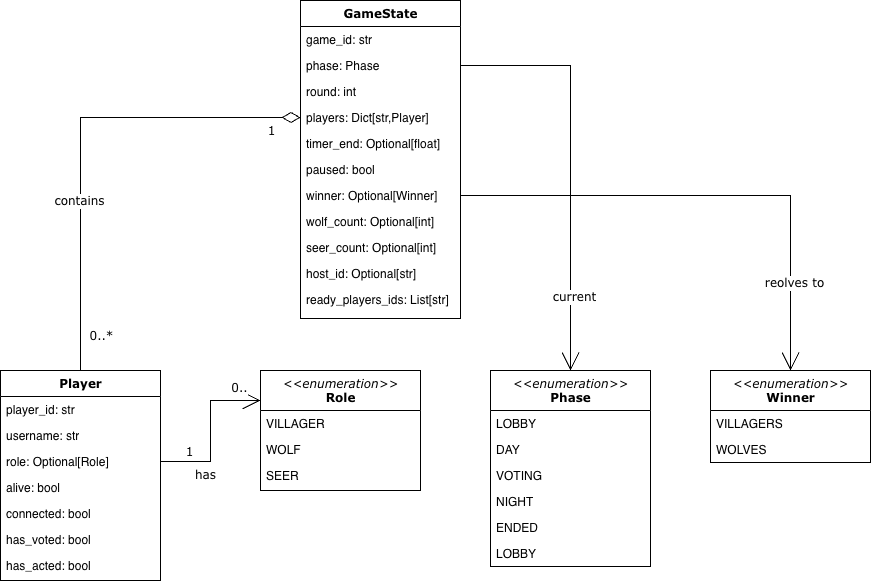
\includegraphics[width=0.75\textwidth]{figures/class_diagram.png}
      \caption{Domain class diagram: the room owns players, game state, ballots, and
            the phase timer; roles and phases are enumerations.}
      \label{fig:class}
\end{figure}

\paragraph{Mapping entities to infrastructure.}
All authoritative entity state lives in the shared store, namespaced per room and
scoped under a room-level key (no query ever spans multiple rooms except the
lobby list); nothing authoritative lives in a replica's memory. Clients hold only
a \emph{view}: a local copy of the last received snapshot/events used for
rendering, partitioned into three reactive stores --- a \emph{lobby store} (room
code, players, host, ready set, role setup), a \emph{game store} (phase machine,
own role, phase timer, vote tally, pause state, outcome), and a \emph{chat store}
(messages, active channel, seen-message-id set for de-duplication). Replicas hold
only \emph{ephemeral operational} state --- the registry of locally connected
sockets and the in-memory phase-timer tasks --- reconstructible and tolerated to
be lost (\cref{fault-tolerance}). Chat messages are the one entity deliberately
\emph{not} stored anywhere. All stored state carries a time-to-live measured in
hours, so abandoned rooms garbage-collect themselves.

\paragraph{Domain events and message sorts.}
The system is event-sourced at the \emph{interaction} level (not at storage
level): every relevant fact is a named event --- room membership (player joined,
left, host changed, kicked), lobby (settings updated, ready changed, game start),
game progression (role assigned [private], phase changed, vote update, player
eliminated/killed, no elimination, seer result [private], game ended),
synchronisation (full authoritative snapshot), and system (chat message, error).
Three sorts of messages are exchanged: \textbf{Commands} (client $\to$ server:
cast vote, wolf vote, seer action, update settings, set ready, start, kick,
restart) are validated against authoritative state and can be rejected (an
\emph{error} event answers the issuer only); \textbf{Events} (server $\to$
clients, and server $\to$ server via the bus) notify state changes --- events
between replicas carry an envelope with a unique id, room id, \emph{sender replica
      id} (for deduplication), timestamp, and optionally a \emph{target client id}
marking a private unicast; \textbf{Queries} (lobby list, health) never modify
state and can be answered by any replica. Separating commands (intents, which may
fail) from events (committed facts) keeps the authorization logic of
\cref{security} straightforward.

\subsection{Interaction}\label{interaction}

Interaction combines four patterns, each used where its coupling fits.

\paragraph{Request/response} is used only for queries (lobby list, health checks)
and for serving static assets, plus a single REST call to fetch the initial game
state when entering the game screen. Any replica can play the responder role.

\paragraph{Publish/subscribe, twice.}
The core gameplay flow enacts publish/subscribe at two nested levels:
\begin{enumerate}
      \item \emph{client-facing}: joining room $R$ subscribes a client to $R$'s event
            stream over its persistent connection; the serving replica is the broker for
            its local subscribers;
      \item \emph{replica-facing}: each replica subscribes to the bus channel of
            every room for which it currently hosts at least one client (unsubscribing when
            its last local member leaves). Every event a replica produces is both emitted
            to its local subscribers \emph{and} published on the room channel.
\end{enumerate}
A replica receiving a bus message relays it to its local room members ---
\emph{unless} the message's \emph{sender id} is its own, in which case it drops it
(sender-based \textbf{deduplication}), preventing the double delivery that would
otherwise occur on the originating replica. Local emission is done before/besides
publication on purpose: clients on the originating replica get minimal latency,
and a bus outage degrades cross-replica delivery only (\cref{fault-tolerance}).
An important client-side rule complements this: the client \emph{never assumes
      its command succeeded} until it receives the corresponding confirmation event ---
casting a vote does not update the local tally directly; the tally updates only
when the server broadcasts the \texttt{vote\_update}. \Cref{tab:events}
summarises the event contract.

\begin{table}
      \centering
      \small
      \begin{tabular}{@{}p{2.0cm}p{6.0cm}p{5.2cm}@{}}
            \toprule
            \textbf{Scope}                                                                                                                                                                                                                                                                                   & \textbf{Received (server $\to$ client)} & \textbf{Emitted (client $\to$ server)} \\
            \midrule
            Lobby                                                                                                                                                                                                                                                                                            &
            \texttt{game\_state\_sync}, \texttt{player\_joined}, \texttt{player\_left}, \texttt{player\_ready}, \texttt{role\_setup\_updated}, \texttt{room\_closed}, \texttt{kicked}                                                                                                                        &
            \texttt{lobby:player\_ready}, \texttt{lobby:update\_settings}, \texttt{lobby:start\_game}, \texttt{kick\_player}                                                                                                                                                                                                                                                                    \\
            \addlinespace
            Game                                                                                                                                                                                                                                                                                             &
            \texttt{game\_start} / \texttt{start\_game}, \texttt{phase\_changed}, \texttt{role\_assigned}, \texttt{vote\_update}, \texttt{player\_eliminated}, \texttt{player\_killed}, \texttt{seer\_result}, \texttt{no\_elimination}, \texttt{game\_ended}, \texttt{game\_paused}, \texttt{game\_resumed} &
            \texttt{cast\_vote}, \texttt{wolf\_vote}, \texttt{seer\_action}, \texttt{return\_to\_lobby}                                                                                                                                                                                                                                                                                         \\
            \addlinespace
            Chat                                                                                                                                                                                                                                                                                             &
            \texttt{chat\_message}                                                                                                                                                                                                                                                                           &
            \texttt{chat\_message}                                                                                                                                                                                                                                                                                                                                                              \\
            \bottomrule
      \end{tabular}
      \caption{Socket.IO event contract between client and server (exact names shared
            with the backend).}
      \label{tab:events}
\end{table}

The typical fan-out of a game action (a vote) is: (1) client $C_1$ on replica $A$
sends the \emph{cast vote} command; (2) $A$ validates it against the store,
records the vote atomically, and builds the \emph{vote update} event; (3) $A$
emits it to its local room members and publishes it on the room channel; (4)
replica $B$ receives it from the bus, sees a foreign sender id, and relays it to
its local members (e.g.\ client $C_2$); (5) both $C_1$ and $C_2$ render the same
vote within milliseconds (\cref{fig:sequence}).

\begin{figure}
      \centering
      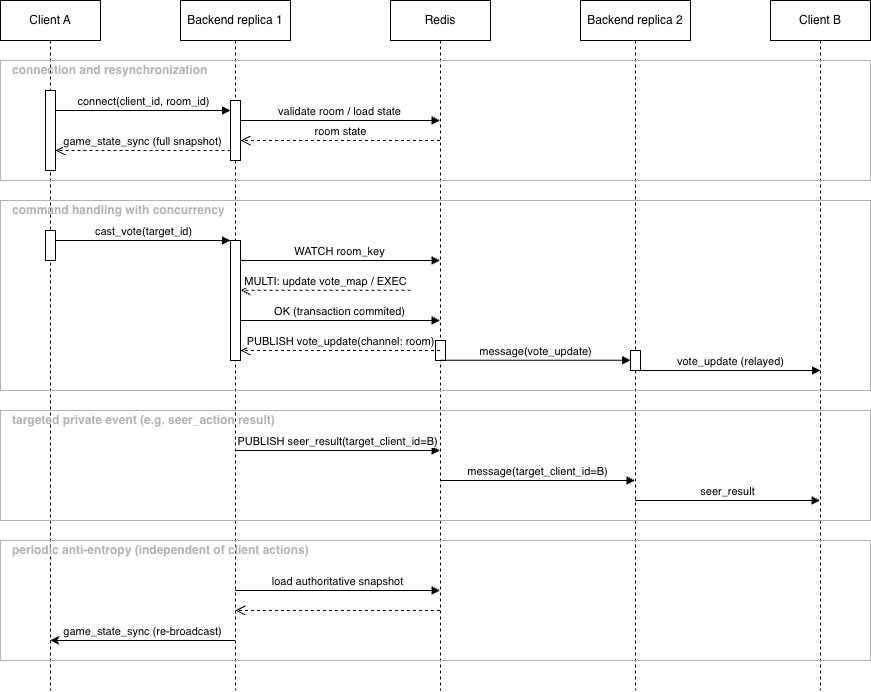
\includegraphics[width=\textwidth]{figures/sequence_diagram.png}
      \caption{Sequence diagram of a cross-replica game action. The originating
            replica writes the shared store atomically, emits to its own clients
            immediately, and publishes on the room channel; another replica relays the
            event to its local clients, while the originator discards the copy the bus
            echoes back to it (sender-based deduplication).}
      \label{fig:sequence}
\end{figure}

\paragraph{Cross-replica unicast} handles \emph{private} events (role
assignment, seer result), which must reach exactly one client whose location the
producer does not know. The event is emitted directly if the target's socket is
local, \emph{and} published with the \emph{target client id} set: each replica
receiving it delivers it only if it currently hosts that client's socket, and
never broadcasts it. This preserves both location transparency and secrecy (FR5,
FR8).

\paragraph{Periodic anti-entropy broadcast.}
Because the bus offers at-most-once delivery (\cref{fault-tolerance}), a
time-driven interaction complements the event flow: every few seconds each
replica re-derives the authoritative snapshot of its active rooms and broadcasts
it as a \emph{game state sync} event. Clients treat snapshots as absolute truth,
overwriting their local view --- so any missed event is repaired within one
period (NFR3). The same snapshot is sent point-to-point to every (re)connecting
client as the first message (after it supplies its \texttt{client\_id} and
\texttt{room\_id} in the handshake), making reconnection and initial join the
same code path (FR11).

\subsection{Behaviour}\label{behaviour}

\paragraph{The match as a replicated state machine.}
A match evolves through the phase state machine
\[
      \textsc{lobby} \rightarrow \textsc{night} \rightarrow \textsc{day}
      \rightarrow \textsc{voting} \rightarrow \textsc{night} \rightarrow \cdots
      \rightarrow \textsc{ended} \; (\rightarrow \textsc{lobby}),
\]
where the \textsc{voting}$\to$\textsc{night} transition resolves the public
lynching, the \textsc{night}$\to$\textsc{day} transition resolves the wolf kill
and the seer inspection, every resolving transition runs the win check (possibly
short-circuiting to \textsc{ended}), and the host may loop an ended match back to
the lobby. Transitions are triggered by \emph{either} the phase deadline expiring
\emph{or} the phase completing early (all living players voted; all wolves and the
seer acted) \emph{or} a decisive disconnection.

\begin{figure}
      \centering
      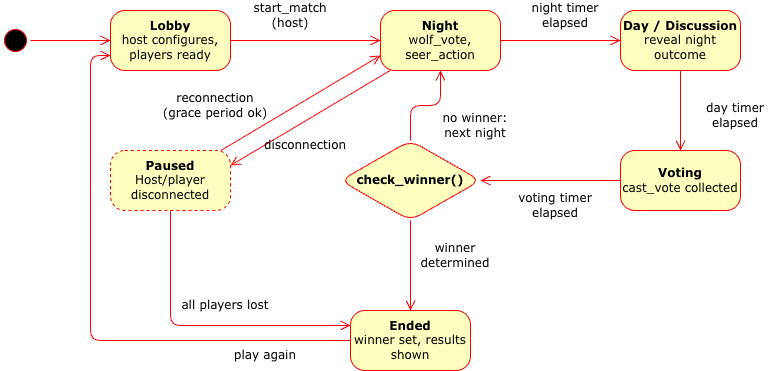
\includegraphics[width=0.85\textwidth]{figures/state_diagram.png}
      \caption{State diagram of a match: the phases and the transitions that resolve
            the public lynching, the night actions, and the win check, up to the
            \textsc{ended} state and the optional loop back to the lobby.}
      \label{fig:state}
\end{figure}

\paragraph{Backend replicas (stateless, reactive).}
Each replica is a purely reactive component: it responds to client commands, bus
messages, connection lifecycle events, and two internal clocks. Since replicas
keep no authoritative state, \emph{any} replica can process \emph{any} trigger
for \emph{any} room --- correctness is delegated to the store's atomic operations
rather than to replica identity. The two internal clocks are:
\begin{itemize}
      \item the \emph{phase timers}: when a replica performs a transition it
            schedules an in-memory timer for the new deadline (the absolute deadline is
            stored authoritatively). Timers are a local optimisation, not a correctness
            mechanism: a firing timer checks the \emph{stored} deadline first and aborts if
            the phase has meanwhile advanced elsewhere (stale-timer guard);
      \item the \emph{sweeper}: every couple of seconds each replica scans the
            active-rooms registry for matches whose stored deadline has passed and advances
            them --- so phase progression survives the death of the replica that held the
            in-memory timer (NFR2).
\end{itemize}
Both paths (and explicit client-triggered advancement) funnel into a single
advancement routine guarded by a short-TTL \emph{distributed lock} acquired
atomically in the store: exactly one trigger wins per deadline, so concurrent
triggers on different replicas cannot double-advance a phase or eliminate two
players (NFR4). The lock is released explicitly on completion through an atomic
compare-and-delete (a Lua script that removes the key only if this replica still
owns it), so a replica can never release a competitor's lock. Its short TTL
(10\,s, far below any phase duration) is only a safety fallback should the holder
crash mid-advancement.

\paragraph{Clients (stateful views).}
The client keeps a local replica of the room view and applies events
optimistically; on any \emph{game state sync} it discards its view and adopts the
snapshot. Its stores are \emph{stateful} (each registers listeners once and
updates reactive state per incoming event), while views and visual components are
effectively \emph{stateless} (a screen is a pure function of store state); no
client component ever writes authoritative game state. On disconnection the
client re-connects with the same identity and is treated as a rejoin: mid-game it
re-receives its secret role privately and the current snapshot; in the lobby it
simply re-enters.

\paragraph{Disconnection: pause, grace, resume.}
On the server side, a disconnection during a match marks the player
\emph{disconnected} but keeps them alive, \emph{pauses} the match, and starts a
bounded \emph{grace timer} (20\,s by default, configurable). The player may
reconnect to \emph{any} replica --- which cancels the timer (the expiry handler
also re-checks the store's \emph{connected} flag to cover a reconnection landing
on a different replica) --- and resume their seat, so a transient network drop does
not cost the match. Host promotion is \emph{deferred} while the grace timer is
pending, so a returning host reclaims its role; only if the timer expires without
a reconnection is the player marked as having \emph{fled} --- treated as an
elimination, to avoid stalling phase-completion checks --- after which the match
resumes and the win check is re-run (FR9, FR11, FR12). A player who was already
eliminated (a spectator) leaving triggers an immediate host promotion and win
check without pausing. On the client, this manifests as automatic reconnection, a
pause banner while the server signals \texttt{game\_paused}, and a full resync on
\texttt{game\_resumed}.

\paragraph{Who updates the state.}
Only backend replicas write to the store, and only in reaction to validated
commands or owned transitions; every write is atomic
(\cref{data-and-consistency-issues}). Clients never write state --- they send
commands and render events. The proxy and monitoring components are stateless
with respect to the domain.

\subsection{Data and Consistency Issues}\label{data-and-consistency-issues}

\paragraph{What is stored, and why key--value.}
All data of \cref{modelling} is stored in the shared in-memory store as
JSON-serialised values under a per-room key namespace: a string key per room
snapshot and per game-state record, hashes for the player registry and the
ballots (field = player id), a string for the phase deadline, and a set for the
active-rooms registry, all with a six-hour TTL renewed on write. A
key--value/hash model fits naturally: the data is small, schema-light, always
accessed by known key, and never queried relationally --- there are no joins, no
secondary indexes, no cross-room queries except the lobby list, served by an
incremental \texttt{SCAN} of the room-snapshot namespace. A relational or
document database would add operational weight (IR3) and millisecond-scale
latency to a path hit several times per game action. Durability requirements are
modest (game state is ephemeral), so an in-memory store with lightweight disk
persistence (periodic snapshots plus an append-only log fsynced every second) is
an appropriate trade-off: after a store crash, at most the last second of updates
is lost --- at worst, re-casting a vote.

\paragraph{Who reads and writes.}
Only backend replicas access the store; the frontend never talks to it directly,
which keeps every mutation subject to the authorization checks of
\cref{security}. Reads happen on every command validation, on every (re)connection
(snapshot), on the sweeper/anti-entropy scans, and on lobby-list queries; writes
on membership changes, lobby reconfiguration, votes and night actions, and phase
transitions. The same room's state is routinely accessed by several replicas at
once (their clients act simultaneously): concurrent reads and writes are the
normal case, not an edge case, which is precisely where the consistency issues
below arise.

\paragraph{Consistency strategy: strong at the store, eventual at the clients.}
The design splits the consistency question in two:
\begin{itemize}
      \item \textbf{Authoritative state} must never violate the game invariants
            (NFR4). All multi-step updates are made \emph{atomic at the store}, which acts
            as the single serialisation point: every replica's writes are applied in one
            total order, so lost updates are prevented by construction rather than by
            inter-replica coordination. Four mechanisms are used, in increasing strength:
            (1) \emph{single-operation atomicity} for naturally atomic updates (a vote is
            one hash-field write); (2) \emph{atomic create-if-absent} (\texttt{SET NX}) for
            room bootstrap --- when two strangers create the same room simultaneously on
            different replicas, only one initial-state write succeeds and its author becomes
            host, eliminating the ``double host'' race (FR1); (3) \emph{optimistic
                  transactions} (\texttt{WATCH}/\texttt{MULTI}, watch--modify--retry) for
            read-modify-write patches of the game-state record, aborting and retrying on a
            concurrent modification instead of silently overwriting it, each successful
            patch bumping the \emph{state version}; (4) \emph{mutual exclusion} where an
            entire multi-key procedure must run at most once per deadline --- the phase
            advancement lock of \cref{behaviour}.
      \item \textbf{Client views} are only \emph{eventually
                  consistent}~\cite{vogels2009eventually}: an event can reach clients of different
            replicas at slightly different times, or be missed entirely (at-most-once bus).
            The design accepts this --- sub-second divergence is imperceptible in a
            chat-paced game --- and guarantees \emph{convergence} instead: the periodic
            anti-entropy snapshot (\cref{interaction}) overwrites any diverged view within
            seconds (NFR3), toward the correct value since snapshots are recomputed from
            authoritative state.
\end{itemize}
This split is the project's answer to the CAP trade-off~\cite{gilbert2002brewer}:
rather than paying for consensus among
replicas~\cite{fischer1985impossibility}, the design concentrates consistency in
one store and treats replicas as caches holding no divergable copy of domain
state at all.

\paragraph{Client-side de-duplication.}
Because a client can receive the same event through more than one path (its
originating replica's local emit plus a relay, or a re-broadcast after
reconnection), the chat store de-duplicates messages by tracking already-seen
message identifiers, so a duplicated delivery is rendered only once --- a
concrete client-side accommodation of the underlying at-least-once delivery that
multi-path fan-out produces.

\paragraph{Shared data between components.}
Beyond domain state, replicas share only two coordination artefacts, both in the
store: the active-rooms set (work list for sweeper/anti-entropy) and the
advancement locks. Notably, replicas do \emph{not} share their connection
registries: which client is connected to which replica is kept local, and
cross-replica delivery is solved by publish/subscribe semantics instead of by a
shared session directory --- one less piece of shared mutable state to keep
consistent.

\subsection{Fault-Tolerance}\label{fault-tolerance}

The failure model is crash (fail-stop) of any single server-side process, plus
message loss: the inter-replica bus provides \emph{at-most-once} delivery, and
the network is assumed unreliable in all the classic
ways~\cite{rotem2006fallacies}.

\paragraph{Replication and redundancy.}
The \emph{service} is actively replicated ($\geq 2$ identical replicas,
active--active): any replica serves any room, so a crash removes capacity but no
function. \emph{Data} is not replicated across nodes (single store); it is made
recoverable by the store's own disk persistence (snapshot + append-only log),
restoring state on restart with at most one second of loss. This asymmetry is
deliberate: replicating the stateless service is cheap, replicating the store
safely is not (primary election and failover), and the dependability requirement
--- do not lose running matches --- is met already if the store's downtime is
short, because all other components mask it.

\paragraph{Heart-beating, timeouts, retries.}
Failure detection is timeout-based at every seam:
\begin{itemize}
      \item \emph{orchestrator} $\to$ \emph{replicas}: liveness probes restart a
            wedged replica; readiness probes remove a replica from load balancing until it
            can actually serve (connected to the store), so clients are never routed to a
            half-alive instance;
      \item \emph{clients} $\leftrightarrow$ \emph{replicas}: the realtime protocol
            exchanges application-level heartbeats; a client detecting a dead connection
            reconnects automatically (through the balancer, hence possibly to a
            \emph{different} replica) and is re-synced by snapshot;
      \item \emph{replicas} $\to$ \emph{store}: every publish is retried a bounded
            number of times with exponential back-off before being declared lost; the bus
            \emph{listener} detects connection failure and enters an unbounded reconnect
            loop with capped back-off, re-subscribing all its channels once the store
            returns --- without this a store blip would silently and permanently cut a
            replica off the bus;
      \item \emph{proxy} $\to$ \emph{replicas}: connect/read timeouts plus
            request-time DNS re-resolution route around dead replicas.
\end{itemize}

\paragraph{What happens when each component fails.}
\begin{description}
      \item[A backend replica crashes.] Its clients' connections drop; they reconnect
            through the balancer to surviving replicas and receive the authoritative
            snapshot --- nothing is lost because the replica held nothing authoritative. Its
            in-memory timers die with it: the cross-replica sweeper notices the expired
            stored deadline within a couple of seconds and advances the match on another
            replica, under the advancement lock (NFR2).
      \item[The store becomes unreachable.] Commands requiring state fail cleanly
            (clients get error events and can retry); already-delivered views remain
            rendered, so ongoing discussion is not interrupted. Each replica's listener
            keeps retrying; on recovery, publishes resume, channels are re-subscribed, and
            the next anti-entropy round re-syncs every client. Events lost on the bus during
            the outage are repaired by the same mechanism --- the design never assumes bus
            reliability, only store reliability \emph{over time}.
      \item[The proxy or frontend crashes.] Both are stateless; the orchestrator
            restarts them, and clients experience a transient connection error. The
            monitoring stack is entirely out of the game's fault path.
\end{description}

\begin{table}
      \centering
      \footnotesize
      \setlength{\tabcolsep}{6pt}
      \renewcommand{\arraystretch}{1.3}
      \caption{Failure modes and how the platform tolerates them. Detection is
            timeout-based at every seam; recovery never depends on the failed component
            itself, and the fault of any single server-side component leaves running
            matches intact.}
      \label{tab:failure-modes}
      \begin{tabular}{@{}
            >{\raggedright\arraybackslash}p{2.4cm}
            >{\raggedright\arraybackslash}p{3.1cm}
            >{\raggedright\arraybackslash}p{4.8cm}
            >{\raggedright\arraybackslash}p{2.6cm}@{}}
            \toprule
            \textbf{Failure} & \textbf{Detected by}                                                       & \textbf{Recovery}
                             & \textbf{Player impact}                                                                         \\
            \midrule
            Backend replica crash
                             & orchestrator liveness/readiness probes; client heartbeat
                             & clients reconnect through the balancer to a surviving replica and re-sync
            by snapshot; the sweeper advances the phase timer under the advancement
            lock
                             & brief reconnect; match continues (NFR2)                                                        \\
            Store (Redis) unreachable
                             & Pub/Sub listener error; failed store commands
                             & listener reconnect loop with back-off $+$ channel re-subscription; publish
            retries; anti-entropy re-syncs every client on recovery
                             & state-changing commands rejected briefly; rendered views persist                               \\
            Proxy / frontend crash
                             & orchestrator liveness probe
                             & stateless restart; request-time DNS re-resolution routes around it
                             & transient connection error, auto-reconnect                                                     \\
            Client disconnect / network drop
                             & socket close $+$ missed heartbeats
                             & match paused, grace timer started; reconnect (to any replica) resumes it,
            otherwise the player is dropped
                             & short pause; resumes on return                                                                 \\
            Monitoring stack down
                             & Prometheus self-monitoring / alerts
                             & stateless restart
                             & none (observability only)                                                                      \\
            \bottomrule
      \end{tabular}
\end{table}

\paragraph{Error handling within the protocol.}
Invalid or unauthorised commands (wrong phase, non-host configuration attempt,
dead voter) are rejected by validation against authoritative state and answered
with a private \emph{error} event --- misbehaving or buggy clients cannot corrupt
state. Unexpected exceptions in event handlers are caught per-event: one
malformed message cannot take down a replica's event loop. Corrupted records read
from the store (failed deserialisation) are logged and skipped rather than
crashing the reader.

\subsection{Availability}\label{availability}

\paragraph{Caching.}
There is no cache tier by design: the store is itself in-memory with
sub-millisecond access, so a cache in front of it would add a consistency problem
without a latency benefit. Two cache-like mechanisms exist nonetheless: the
per-room \emph{snapshot} record is a denormalised, ready-to-send materialised
view (refreshed on every relevant change and by anti-entropy), so client
synchronisation is one read; and each \emph{client} caches the room view locally
between events, keeping the UI responsive during a brief server-side outage.
Static SPA assets are served with standard HTTP caching.

\paragraph{Load balancing.}
Load balancing happens at connection granularity at the entry proxy: new realtime
connections are assigned to backend replicas \emph{round-robin}. Round-robin is
right for long-lived connections: each connection is a lasting resource
commitment, so the goal is to spread \emph{connection counts} evenly; latency-aware
policies were rejected because a persistent connection produces no response-time
signal until it closes. Because clients reconnect through the balancer, load
\emph{re}-balances naturally after failures and scale-ups. Horizontal elasticity
complements balancing: replicas scale automatically between a floor of 2 (fault
tolerance) and a ceiling of 8, scaling up aggressively on load spikes and down
slowly --- draining a replica disconnects its clients, so scale-down is damped to
once a minute after a 5-minute stabilisation window (NFR5, NFR8). The ceiling of
8 is a pragmatic cap rather than a hard limit: past a point the real bottleneck
becomes the single Redis instance shared by every replica as both state store and
bus, so adding backends only shifts pressure onto it. Eight replicas --- at
roughly 80 concurrent WebSocket connections per replica, some 640 simultaneous
players --- comfortably exceed the load a casual party game must sustain while
staying within the single-machine, zero-budget target (minikube, IR3). Lifting
the ceiling meaningfully would first require a highly available store
(\cref{future-works}).

\paragraph{Behaviour under network partition.}
Applying CAP~\cite{gilbert2002brewer} per partition scenario, the system fails
soft rather than closed:
\begin{description}
      \item[Client partitioned from the cluster.] The match goes on: phases advance
            server-side regardless of individual clients (timers are authoritative), and
            the partitioned player's inaction is handled by the same rules as any inaction;
            on prolonged disconnection the player is marked as having fled. On heal the
            client re-syncs by snapshot --- rebuilding from the snapshot, never from any
            locally cached delta. This favours availability for the \emph{group} over the
            individual, the correct choice for a party game.
      \item[Replica partitioned from the store.] The replica keeps its clients
            connected but refuses state-changing commands (it cannot validate them): it
            degrades to read-only availability on stale views rather than guessing --- for
            authoritative writes the design chooses consistency over availability, because a
            wrong elimination is worse than a delayed one. Its readiness probe fails, so the
            balancer stops routing \emph{new} connections to it. Phase timers are protected
            by comparing the locally scheduled deadline against the stored deadline before
            acting, preventing a previously-partitioned replica from advancing a phase
            twice.
      \item[Split between replicas (bus unreachable, store reachable).] Impossible to
            sustain silently in this topology (bus and store are the same component), but
            the at-most-once analysis of \cref{fault-tolerance} covers transient versions:
            views diverge for at most one anti-entropy period, then converge. Writes remain
            correct throughout, since they serialise at the store.
\end{description}
Independently of any partition scenario, the Kubernetes deployment is configured
for backend high availability: two replicas, rolling updates without downtime,
and readiness/liveness/startup probes together with a \texttt{preStop} hook that
drains in-flight connections before a pod is terminated (NFR2, NFR8).

\subsection{Security}\label{security}

\paragraph{Authentication.}
There is no account system: players self-identify with a nickname scoped to a
room (a \texttt{client\_id} generated and stored client-side, passed in the
Socket.IO handshake), which doubles as their client identifier. This is a
conscious trade-off (\cref{ds-features}): the product is a casual party game, no
sensitive data is at stake, and login friction would hurt the primary use case
more than impersonation would. The nickname is weakly protected where it matters
for gameplay: a name already connected to a room cannot be taken by a second
connection (preventing casual impersonation and accidental double tabs, FR14),
and the same identity lets a disconnected player resume their seat (FR11).

\paragraph{Authorization.}
Access control is enforced \emph{server-side on every command}, on authoritative
state, never on client claims. It is a small role-based scheme with three axes:
\emph{platform role} (host-only rights --- configure, start, kick, restart ---
checked against the stored host identity); \emph{game role and liveness} (only
living players may vote; only wolves may wolf-vote; only the seer may inspect;
spectators retain read access only); and \emph{phase} (every command is valid
only in its phase --- configuration in \textsc{lobby}, votes in \textsc{voting},
night actions in \textsc{night}), which blocks whole classes of out-of-order
exploits. On the client, chat channels are filtered by role/liveness and action
controls are enabled only for the eligible role in the correct phase --- but this
client-side filtering is a UX safeguard only; the authoritative enforcement is
server-side. Information-flow control complements access control: secret data
(roles, wolf ballots, seer results) is delivered only over private unicast events
and is systematically excluded from broadcast snapshots until game end --- so even
a modified client observing all its traffic learns nothing it should not (FR5,
FR8).

\paragraph{Perimeter and cryptography.}
The proxy is the only exposed component; internal components are on segregated
networks and unreachable from outside (\cref{infrastructure}). It applies per-IP
rate limits (separate budgets for API calls and connection attempts) to blunt
abuse and trivial denial-of-service, sets standard security headers, and hides
implementation details. No custom cryptographic schema is used --- there are no
passwords or tokens to protect, and transport encryption (TLS) is a deployment
concern the proxy is already prepared for (port 443 is reserved; the local course
deployments run plain HTTP). Interactive API documentation is disabled outside
development.

\section{Implementation}\label{implementation}

This section binds the design of \cref{design} to concrete technologies,
motivating each choice.

\subsection{Network protocols}\label{network-protocols}

Two application-level protocols are used, one per interaction kind of
\cref{interaction}. Client--server realtime communication uses
\textbf{Socket.IO}~\cite{socketio} on top of WebSocket (over TCP/HTTP).
Socket.IO was preferred to raw WebSocket because it provides out of the box
exactly the machinery the design requires: named events, \emph{rooms} (the
per-room topic abstraction), application-level heartbeats (ping/pong) for
failure detection, and automatic client reconnection with back-off ---
re-implementing these reliably over raw WebSocket is error-prone and out of
scope. The HTTP long-polling fallback that Socket.IO offers is deliberately
\emph{disabled} on the client (WebSocket-only transport), to keep a single,
clean upgrade path behind the reverse proxy. Queries (lobby list, health) and
the single initial-state fetch use plain \textbf{HTTP/1.1} REST endpoints.

Between backend replicas, synchronization reuses neither Socket.IO nor HTTP: it
happens over \textbf{Redis Pub/Sub}, i.e.\ the Redis serialization protocol
(RESP) over TCP, the same connection already used for state
persistence~\cite{redis}. Reusing the existing Redis connection for both state
and cross-replica notification avoids introducing a separate message broker,
which would add an infrastructural component and a failure mode without a
corresponding benefit at this scale. The backend runs as a single ASGI process
exposing both the REST and the Socket.IO surface; the proxy upgrades WebSocket
connections (\texttt{Upgrade}/\texttt{Connection} headers) and keeps them alive
with hour-long read timeouts.

\subsection{In-transit data representation}\label{in-transit-data}

All payloads --- client events, bus messages, stored values --- are
\textbf{JSON}. The dominant consumer is a browser, so JSON is the zero-friction
choice, and Socket.IO is built around JSON-friendly payloads on the JavaScript
side. Payloads are small (well under the enforced 1\,MB cap) and exchanged at
most a handful of times per second per room, so a binary format (Protocol
Buffers, MessagePack) would buy little except schema tooling on both the Python
backend and the Vue frontend. Using the same representation for the wire format
and for the Redis-persisted state also lets a payload be stored and broadcast
without an intermediate transformation. Message \emph{schemas} are nonetheless
explicit in code: every event family has a typed model --- Pydantic models for
the \texttt{RedisEvent} bus envelope (event id, type, room, sender replica,
timestamp, payload, optional target client) and the \texttt{WSMessage} client
envelope, plus dataclasses per event payload converted to JSON-serializable
dictionaries before emission --- so malformed messages are rejected at the
boundary rather than deep in game logic.

\subsection{Database querying}\label{database-querying}

The store is \textbf{Redis 7}~\cite{redis}, accessed through its native
asynchronous Python client (\texttt{redis.asyncio}) --- no ORM and no SQL, since
the data model is key--value by design (\cref{data-and-consistency-issues}). All
interaction is NoSQL: key--value and hash operations (\texttt{GET},
\texttt{SETEX}, \texttt{SET NX EX}, \texttt{HGET}, \texttt{HGETALL},
\texttt{HSET}, \texttt{SADD}, \texttt{SMEMBERS}), combined with
\texttt{WATCH}/\texttt{MULTI}/\texttt{EXEC} transactions for read-modify-write
sequences and a Lua script for atomically releasing the phase-advancement lock.
The consistency mechanisms of \cref{data-and-consistency-issues} map to Redis
primitives one-to-one: atomic creation is \texttt{SET NX EX}; optimistic
transactions are \texttt{WATCH}/\texttt{MULTI}/\texttt{EXEC} retried on
\texttt{WatchError}; the advancement lock is \texttt{SET NX} with a 10\,s TTL
released by the compare-and-delete Lua script; bulk player updates use pipelines
(one round-trip instead of $O(n)$); the lobby list uses cursor-based
\texttt{SCAN} rather than the blocking \texttt{KEYS}. TTLs
(\texttt{SETEX}/\texttt{EXPIRE}, 6\,h, renewed on write) delegate garbage
collection of abandoned rooms to Redis instead of a scheduled task, keeping
replicas as stateless as possible. Pub/Sub channels are named
\texttt{game:\{room\_id\}} plus one global channel.

\subsection{Authentication}\label{impl-authentication}

As designed in \cref{security}, there is no OAuth/JWT machinery. The client
generates (or retrieves, if already present) a \texttt{client\_id}, stores it in
\texttt{sessionStorage}, and sends it --- together with the room id --- in the
Socket.IO connection handshake; the backend treats this identifier as a session
identity rather than a cryptographic credential, binding it server-side to the
socket id via the connection manager. This is a deliberate simplification,
adequate for the controlled, ephemeral environment the game runs in; it would
need to be replaced by a real authentication mechanism before the system could be
exposed where impersonating another player's \texttt{client\_id} carried real
consequence.

\subsection{Authorization}\label{impl-authorization}

Authorization is implemented as guard clauses at the top of every command
handler, reading the authoritative Redis state (host id, phase, role, liveness)
and raising domain errors that reach the offending client as private
\emph{error} events. At the lobby level, only the host may update settings or
start the match. During a match, gameplay actions are enabled only in the phase
they belong to and only for entitled players: \texttt{cast\_vote} is accepted
only during \textsc{voting}, while \texttt{wolf\_vote} and \texttt{seer\_action}
are accepted only during \textsc{night} and only from players holding the
corresponding role, with additional checks that the player is still alive and has
not already acted in the current phase. An RBAC framework would be
over-engineering for three roles and a dozen rules.

\subsection{Technological details}\label{technological-details}

\paragraph{Backend: Python 3.12, FastAPI, python-socketio, Uvicorn.}
The backend is an ASGI application composed of \textbf{FastAPI}~\cite{fastapi}
(REST endpoints, dependency-injected settings via \texttt{pydantic-settings},
OpenAPI docs in development) and \textbf{python-socketio}'s \texttt{AsyncServer}
mounted on the same server, run by \textbf{Uvicorn} with the \texttt{uvloop}
event loop. An asynchronous single-threaded runtime is the natural match for the
workload (\cref{ds-features}): thousands of mostly idle sockets multiplexed over
one event loop, with I/O-bound handlers awaiting Redis. Each container runs
\emph{one} Uvicorn worker --- scaling is horizontal at the container level
(\cref{deployment}), which keeps per-process state (connection registry, timers)
trivially consistent and lets the orchestrator own scaling. Long-running concerns
(Pub/Sub listener, timer sweeper, anti-entropy) are \texttt{asyncio} background
tasks started in FastAPI's lifespan hook. Each replica identifies itself with an
\texttt{INSTANCE\_ID} taken from the \texttt{HOSTNAME} environment variable (the
pod/container name), implementing the sender-id deduplication and lock ownership
of \cref{design} with zero configuration.

\paragraph{Frontend: Vue 3, Pinia, Vue Router, Vite, socket.io-client.}
The SPA uses \textbf{Vue~3} (Composition API, \texttt{<script setup>}), built and
served in development by \textbf{Vite}, with \textbf{Vue Router} mapping four
routes to the four screens (home, lobby, game, results) and \textbf{Pinia} for
state management. The three stores of \cref{modelling} (lobby, game, chat) each
expose reactive state, computed selectors (alive players, own role, whether an
action is currently allowed, the visible chat messages), the event listeners, and
the command-emitting actions. Real-time communication goes through a single
\textbf{socket.io-client} connection shared application-wide (one module-level
instance): WebSocket-only transport; an authentication payload carrying the
\texttt{client\_id} and room id; automatic reconnection with a bounded number of
attempts; and a pending-listener registry that lets stores register handlers
before the socket exists and re-binds them when the connection opens, avoiding
mount/connection races. Listeners are de-registered/re-registered around
reconnections which, combined with message de-duplication
(\cref{data-and-consistency-issues}), prevents duplicated or lost chat messages.
The UI is composed of small reusable components: a player card (SVG with a hidden
back or a revealed role), a deterministic avatar (colour and initials from the
player id), a chat box, a circular phase timer whose colour changes as the
deadline approaches, a role-icon, and an info box. The backend origin is not
baked in at build time: a \texttt{config.js} is generated \emph{at container
      start} by an entrypoint script (\texttt{envsubst} on a template, reading the
\texttt{WS\_URL} environment variable, defaulting to same-origin), so the same
image runs under \texttt{localhost}, \texttt{game.local}, or any production
domain (build-once/configure-at-runtime).

\paragraph{Containerisation.}
Both images are multi-stage builds: the backend separates a
dependency-compilation stage from a slim runtime (\texttt{python:3.12-slim}); the
frontend builds with \texttt{node:20-alpine} and ships only compiled assets on
\texttt{nginx:1.25-alpine}. Both run as non-root users and embed container-level
health checks, yielding small, reproducible, least-privilege images --- the unit
of deployment everywhere from Compose to Kubernetes.

\paragraph{Edge and observability stack.}
The reverse proxy is \textbf{NGINX 1.25} (Compose) and the \textbf{NGINX Ingress
      Controller} (Kubernetes), configured as per \cref{infrastructure,availability}.
Metrics use \texttt{prometheus-fastapi-instrumentator} for HTTP metrics plus
custom counters/histograms (\cref{tab:metrics}), all labelled by
\texttt{instance\_id}; \textbf{Prometheus}~\cite{prometheus} scrapes replicas and
a \texttt{redis\_exporter}, evaluates recording/alert rules (backend down, Redis
down, error rates), and \textbf{Grafana} ships with a provisioned dashboard --- so
observability (NFR7) works out of the box in both deployments.

\begin{table}
      \centering
      \footnotesize
      \setlength{\tabcolsep}{6pt}
      \renewcommand{\arraystretch}{1.25}
      \caption{Custom application metrics exported on \texttt{/metrics} (standard
            HTTP metrics are added automatically by the instrumentator). Every metric
            additionally carries an \texttt{instance\_id} label, so all quantities can be
            broken down per replica; the \emph{Labels} column lists only the further
            dimensions.}
      \label{tab:metrics}
      \begin{tabular}{@{}
            >{\raggedright\arraybackslash}p{5.0cm}
            >{\raggedright\arraybackslash}p{1.6cm}
            >{\raggedright\arraybackslash}p{1.9cm}
            >{\raggedright\arraybackslash}p{4.0cm}@{}}
            \toprule
            \textbf{Metric}                               & \textbf{Type} & \textbf{Labels}      & \textbf{Measures}                         \\
            \midrule
            \multicolumn{4}{@{}l}{\emph{WebSocket connections}}                                                                              \\
            \texttt{ws\_active\_connections}              & Gauge         & ---                  & live WS connections on the replica        \\
            \texttt{ws\_connections\_total}               & Counter       & ---                  & connections accepted since start          \\
            \texttt{ws\_disconnections\_total}            & Counter       & \texttt{reason}      & disconnections (normal / timeout / error) \\
            \addlinespace
            \multicolumn{4}{@{}l}{\emph{WebSocket messages}}                                                                                 \\
            \texttt{ws\_messages\_received\_total}        & Counter       & \texttt{event\_type} & client\,$\to$\,server messages, by event  \\
            \texttt{ws\_messages\_sent\_total}            & Counter       & \texttt{event\_type} & server\,$\to$\,client messages, by event  \\
            \texttt{ws\_message\_size\_bytes}             & Histogram     & ---                  & size of received messages (bytes)         \\
            \addlinespace
            \multicolumn{4}{@{}l}{\emph{Redis Pub/Sub bus}}                                                                                  \\
            \texttt{redis\_messages\_published\_total}    & Counter       & \texttt{channel}     & events published on the bus               \\
            \texttt{redis\_messages\_received\_total}     & Counter       & \texttt{channel}     & events received from the bus              \\
            \texttt{redis\_messages\_deduplicated\_total} & Counter       & ---                  & own-echo events dropped (dedup)           \\
            \texttt{redis\_publish\_failures\_total}      & Counter       & ---                  & publishes lost after all retries          \\
            \texttt{redis\_reconnects\_total}             & Counter       & ---                  & listener reconnects to the store          \\
            \addlinespace
            \multicolumn{4}{@{}l}{\emph{Rooms \& players}}                                                                                   \\
            \texttt{game\_active\_rooms}                  & Gauge         & ---                  & rooms with $\geq 1$ local client          \\
            \texttt{game\_active\_players}                & Gauge         & ---                  & connected players on the replica          \\
            \addlinespace
            \multicolumn{4}{@{}l}{\emph{Internal latency}}                                                                                   \\
            \texttt{redis\_publish\_duration\_seconds}    & Histogram     & ---                  & \texttt{PUBLISH} latency to the broker    \\
            \texttt{ws\_broadcast\_duration\_seconds}     & Histogram     & ---                  & time to broadcast to a room               \\
            \bottomrule
      \end{tabular}
\end{table}

\section{Validation}\label{validation}

Validation combines three layers of automated testing --- unit, integration, and
end-to-end --- with manual acceptance testing of the parts that automated tests do
not cover well. The layers go from pure logic to the deployed system, and
deployment automation (\cref{deployment}) makes it cheap to bring up a
production-like environment to test against.

\subsection{Automatic Testing}\label{automatic-testing}

\subsubsection{Unit testing}\label{unit-testing}

Domain logic and the Redis access layer are unit-tested in isolation, using
\texttt{fakeredis} --- an in-process emulator honouring the same command semantics
--- in place of a real Redis instance, so tests exercise the \emph{real}
data-access code (including transactions) without any running infrastructure:
fast, deterministic, and CI-friendly. On the backend,
\texttt{test\_game\_logic.py} covers role assignment and its validation bounds
(FR3, FR5), phase transitions and their resolutions --- vote tallying with ties
and skips, night kills, seer inspection, win detection (FR6--FR9);
\texttt{test\_lobby\_logic.py} covers host election, ready-state handling, and
lobby rules (FR12); \texttt{test\_state\_store.py} covers persistence and
retrieval through the Redis access layer. The frontend mirrors this with
\textbf{Vitest}: store tests verify how the three Pinia stores react to incoming
events (a \texttt{phase\_changed} updates the phase, a \texttt{vote\_update}
updates the tally, chat de-duplication discards an already-seen message ---
mapping onto FR2--FR8), plus composable/router tests for the countdown and the
route configuration. Views are intentionally not unit-tested: a screen is a pure
projection of store state (already tested) and is better validated end-to-end.
Corner cases live here --- a player with no assigned role yet, an already-expired
phase timer, a match at the minimum player count, an empty initial lobby.

\subsubsection{Integration testing}\label{integration-testing}

A second layer verifies interaction between modules that cooperate on the same
state within a single replica, and the Redis concurrency primitives of
\cref{data-and-consistency-issues} under the conditions they were designed for:
\texttt{test\_lobby\_runtime.py} and \texttt{test\_backend-init.py} check that the
runtime emits the expected events for a given command sequence, while
\texttt{test\_distributed\_safety.py} targets the distributed guarantees directly,
one guarantee per test --- atomic room creation electing exactly one host under a
simulated double-join (FR1, NFR4); the advancement lock admitting a single winner
per room while remaining independent across rooms (NFR4); optimistic patches
merging concurrent field updates and bumping the \texttt{state\_version}
monotonically, i.e.\ no lost updates (NFR4); the active-rooms registry behaving as
the sweeper expects (NFR2); and bulk pipeline persistence preserving per-player
data. These properties are exactly the ones manual testing cannot reliably
exercise: the tests encode the race conditions as deterministic scenarios.

\subsubsection{End-to-end / system testing}\label{e2e-testing}

Standalone Python scripts open genuine Socket.IO/WebSocket connections against a
running backend (Compose with two backend replicas, or the Kubernetes cluster),
exercising the system as a whole rather than through direct function calls, using
the same \texttt{socket.io} client as the real frontend:

\begin{itemize}
      \item \texttt{test\_multi\_instance.py} validates replication transparency
            (NFR1, FR10): events published by a client on replica $A$ reach clients on
            replica $B$ and vice versa, local broadcast still works, and the sender never
            receives its own event twice (deduplication). It can target the load-balanced
            entry point or two specific pods via \texttt{kubectl port-forward}, asserting on
            the \texttt{instance\_id} carried by every message.
      \item \texttt{test\_reconnection.py} validates state synchronisation (FR11,
            NFR3): a fresh room yields no spurious snapshot; a client reconnecting to the
            same or a \emph{different} replica receives the state produced while it was away;
            two clients on different replicas observe consistent state after churn.
      \item \texttt{load\_test.py} validates NFR5/NFR6: a multi-process Socket.IO load
            generator (hundreds of concurrent clients spread over several OS processes, so
            that the bottleneck under test is the platform, not the generator) measures
            connection success and event delivery under load, and is used to observe HPA
            scale-up and connection spreading live (\texttt{kubectl get hpa -w} and the
            Grafana dashboard). A companion diagnostic (\texttt{diag\_loss.py}) distinguishes
            real event loss from test artefacts.
\end{itemize}

The corner cases exercised here include loss or delay of Pub/Sub messages, a
client reconnecting to a different replica, a duplicate-host race, both local and
cross-instance broadcast, bursts of messages in a short window, and disconnection
followed by state recovery. Crash-recovery of phase timers is exercised by killing
a backend pod during a scripted match (the sweeper advances the phase within its
period --- NFR2). Lightweight smoke checks confirm reachability before the more
expensive runs:

\begin{verbatim}
# Smoke checks
curl http://game.local/health
wscat -c "ws://game.local/ws/test_room?client_id=test123"

# Multi-instance propagation (replication transparency)
python tests/test_multi_instance.py --url http://game.local
# Reconnection and state consistency
python tests/test_reconnection.py --url http://game.local
# Message-loss diagnostics
python tests/diag_loss.py ws://game.local/ws
# Load test
python tests/load_test.py --url http://game.local --clients 300 --procs 4
\end{verbatim}

\begin{table}
      \centering
      \small
      \begin{tabular}{p{2.1cm} p{3.4cm} p{4.2cm} p{2.5cm}}
            \toprule
            \textbf{Layer} & \textbf{What it validates}                                                                     & \textbf{Rationale}                                                                    & \textbf{Requirement(s)}        \\
            \midrule
            Unit           & Domain rules, state serialization, UI derivations, in isolation via \texttt{fakeredis} / mocks & Fast, deterministic feedback on pure logic and corner cases                           & Underlies NFR1; FR3--FR9, FR12 \\
            Integration    & Cooperating runtime modules and Redis concurrency primitives on a single replica               & Individually-correct components can still misbehave once combined at sensitive points & FR1, NFR2, NFR4                \\
            End-to-end     & Real network communication, cross-replica propagation, reconnection, load                      & Only observable with a running system, not from function calls                        & NFR1--NFR6, FR10--FR11         \\
            \bottomrule
      \end{tabular}
      \caption{Summary of the automated testing layers.}
      \label{tab:test-summary}
\end{table}

\subsection{Acceptance test}\label{acceptance-test}

Manual play-testing sessions were run on the full deployment for the properties
that resist automation, because they involve several real clients interacting over
the network in real time. Independent client identities were obtained with
multiple browser windows in separate incognito sessions. The scenarios exercised:

\begin{itemize}
      \item \emph{full-game flows}: complete matches with 5+ players including seer
            play, skip votes, mid-game abandonments, kicks, end-game screens, and
            play-again loops (FR4--FR9, FR13) --- automating a whole match with hidden-role
            coordination across many scripted clients was judged poor value, since the
            underlying rules are already unit-tested;
      \item \emph{perceived experience}: UI readability, timer smoothness, and the
            simultaneity of phase changes and eliminations across screens --- qualitative
            judgements (layout, role banners, perceived responsiveness) a script cannot
            make;
      \item \emph{fault and multi-instance scenarios}: transient disconnection and
            reconnection during a match (verifying state resynchronisation), players of the
            same room deliberately spread across two backend replicas (confirming events
            reach everyone and the client behaves identically regardless of routing), and
            operational drills --- killing pods mid-match, restarting Redis, and watching the
            system converge (semi-automated via deployment scripts + dashboards, validated
            by human observation).
\end{itemize}

Each acceptance session mapped observed behaviour back to the acceptance criteria
of \cref{requirements}; all functional requirements were verified on the
Kubernetes deployment before delivery.

\section{Deployment}\label{deployment}

The platform supports three deployment profiles, all driven by files versioned in
the repository; complete step-by-step instructions live in the repository
\texttt{README}. \Cref{tab:profiles} summarises them. They share the same images
and configuration mechanism (\cref{technological-details}) and differ only in what
is containerised and in the target environment.

\begin{table}
      \centering
      \footnotesize
      \setlength{\tabcolsep}{6pt}
      \renewcommand{\arraystretch}{1.25}
      \caption{The three deployment profiles.}
      \label{tab:profiles}
      \begin{tabular}{@{}
            >{\raggedright\arraybackslash}p{2.6cm}
            >{\raggedright\arraybackslash}p{4.2cm}
            >{\raggedright\arraybackslash}p{3.8cm}
            >{\raggedright\arraybackslash}p{2.6cm}@{}}
            \toprule
            \textbf{Profile} & \textbf{Bring-up command}                                                 & \textbf{Brings up}
                             & \textbf{Entry point}                                                                           \\
            \midrule
            \textbf{1 --- Development} \newline \emph{support only, hot-reload}
                             & \texttt{docker compose -f} \texttt{docker-compose-dev.yml up -d}
            \newline $+$ native \texttt{uvicorn --reload} and \texttt{npm run dev}
                             & Redis, exporter, Prometheus, Grafana (backend and frontend run natively)
                             & Vite dev server on \texttt{localhost}                                                          \\
            \addlinespace
            \textbf{2 --- Full Compose} \newline \emph{single machine, full stack}
                             & \texttt{docker compose up -d} \texttt{-{}-scale backend=2}
                             & NGINX, $N$ backend replicas, frontend, Redis, monitoring stack
                             & \texttt{http://localhost}                                                                      \\
            \addlinespace
            \textbf{3 --- Kubernetes} \newline \emph{cluster, production-like}
                             & \texttt{k8s/deploy.sh} \newline (or the documented \texttt{kubectl apply}
            sequence)
                             & namespace, ConfigMap/Secret, Redis $+$ PVC, backend $+$ HPA (2--8),
            frontend, monitoring, Ingress
                             & \texttt{http://game.local} \newline (via \texttt{minikube tunnel})                             \\
            \bottomrule
      \end{tabular}
\end{table}

\subsection{Prerequisites and configuration}\label{prerequisites}

The only host requirements are Docker Desktop 24+ with Compose v2 and, for the
cluster profile, \texttt{kubectl} 1.28+ and \texttt{minikube} 1.32+ (with the
\texttt{ingress} and \texttt{metrics-server} addons). \texttt{Node.js 20} and
\texttt{Python 3.12} are needed only to run or test frontend/backend outside their
containers. These versions match the base images actually used: the backend is
built from \texttt{python:3.12-slim}, the frontend from \texttt{node:20-alpine},
and the infrastructure containers use \texttt{redis:7.2-alpine},
\texttt{prometheus:2.51.0}, and \texttt{grafana:10.4.0}.

All application configuration flows through \emph{environment variables} with
sensible defaults (Redis URL, channel prefix, phase durations, log level), already
defined --- with working values --- directly inside the deployment manifests
(\texttt{docker-compose.yml}, \texttt{docker-compose-dev.yml}, and the
\texttt{k8s/} ConfigMaps). No variable needs to be set by hand and no separate
\texttt{.env} file must be created for a standard installation: running
\texttt{docker compose up} or \texttt{kubectl apply -f k8s/} is enough on its own.
The same images run in every environment (\cref{technological-details}).

\subsection{Profile 1 --- development (support services only)}\label{profile-dev}

\texttt{docker compose -f docker-compose-dev.yml up -d} starts only the
stateful/support services (Redis, its exporter, Prometheus, Grafana), while the
backend (\texttt{uvicorn main:app --reload}) and frontend (\texttt{npm run dev})
run natively with hot-reload:

\begin{verbatim}
docker compose -f docker-compose-dev.yml up -d
cd backend  && pip install -r requirements.txt && uvicorn main:app --reload --port 8000
cd frontend && npm install && npm run dev
\end{verbatim}

This keeps the edit cycle at IDE speed while developing against real
infrastructure; it trades the production-like guarantees of the full stack
(reverse proxy, multiple replicas, containerised frontend) for fast reloads and is
not the final deployment target.

\subsection{Profile 2 --- full Docker Compose}\label{profile-compose}

\texttt{docker compose up -d --scale backend=2} builds and starts the entire
platform on one machine: NGINX (the only published entry point, port 80), $N$
backend replicas, the frontend, Redis, and the monitoring stack. The backend is
explicitly scaled to more than one replica so that the distributed behaviour of
\cref{design} is actually exercised rather than degenerating to a single instance:

\begin{verbatim}
docker compose build
docker compose up -d --scale backend=2
docker compose ps
curl http://localhost/health
\end{verbatim}

The Compose file encodes the design decisions of \cref{infrastructure} directly:
four segregated bridge networks (proxy--frontend, proxy--backend, backend--Redis,
monitoring); named volumes for Redis, Prometheus, and Grafana; health checks on
every service with \texttt{depends\_on: condition: service\_healthy} (backends
start only after Redis answers \texttt{PING}); a replica-friendly backend
definition (no fixed container name or published port, so \texttt{--scale
      backend=$N$} just works, NGINX resolving the service name at request time); and
resource limits mirroring the Kubernetes ones. Expected outcome: every service
\emph{healthy}; the game at \texttt{http://localhost}, the WebSocket endpoint at
\texttt{ws://localhost/ws/<room\_id>}, the REST API under
\texttt{http://localhost/api/}, Prometheus at \texttt{:9090}, Grafana at
\texttt{:3001}; \texttt{curl /health} returns each replica's id in round-robin.

\subsection{Profile 3 --- Kubernetes (minikube)}\label{profile-k8s}

Images are built into minikube's Docker daemon, then either the
\texttt{k8s/deploy.sh} script (or its PowerShell twin) or the documented
\texttt{kubectl apply} sequence deploys, in dependency order --- namespace,
ConfigMap/Secret, Redis (waiting for rollout), backend, frontend, monitoring,
Ingress:

\begin{verbatim}
kubectl apply -f k8s/namespace.yml
kubectl apply -f k8s/configmap.yml
kubectl apply -f k8s/redis/
kubectl apply -f k8s/backend/
kubectl apply -f k8s/frontend/
kubectl apply -f k8s/monitoring/redis-exporter.yml
kubectl apply -f k8s/monitoring/prometheus.yml
kubectl apply -f k8s/monitoring/grafana.yml
kubectl apply -f k8s/ingress.yml
# or, equivalently:
./k8s/deploy.sh
\end{verbatim}

The manifests add production-grade concerns on top of the Compose design
(\cref{tab:k8s}): a backend Deployment with zero-downtime rolling updates and three
probes; an HPA scaling 2--8 replicas; a single Redis with a PersistentVolumeClaim
and \texttt{Recreate} strategy (never two writers on one volume); a
WebSocket-ready Ingress with per-IP limits, plus a \emph{separate} monitoring
Ingress without those limits so dashboards stay reachable during load tests; and
Prometheus rules and the Grafana dashboard injected as ConfigMaps generated from
the same source files used by Compose (a single source of truth). Expected
outcome: \texttt{kubectl get pods -n game} shows \texttt{backend}\,$\times2$,
\texttt{frontend}\,$\times2$, \texttt{redis}, \texttt{redis-exporter},
\texttt{prometheus}, \texttt{grafana} all \texttt{Running}; with
\texttt{minikube tunnel} active and \texttt{game.local} in the hosts file, the
game answers at \texttt{http://game.local}, \texttt{/health} returns \texttt{ok},
and Grafana/Prometheus are reachable under \texttt{/grafana} and
\texttt{/prometheus}. Verify with:

\begin{verbatim}
kubectl get pods -n game
kubectl get services -n game
kubectl get ingress -n game
kubectl get hpa -n game
curl http://game.local/health
\end{verbatim}

\begin{table}
      \centering
      \footnotesize
      \setlength{\tabcolsep}{6pt}
      \renewcommand{\arraystretch}{1.3}
      \caption{Key configuration of the main Kubernetes objects (namespace
            \texttt{game}). Values are taken directly from the manifests; the rationale
            column links each choice to the requirement it serves.}
      \label{tab:k8s}
      \begin{tabular}{@{}
            >{\raggedright\arraybackslash}p{2.8cm}
            >{\raggedright\arraybackslash}p{7.4cm}
            >{\raggedright\arraybackslash}p{3.0cm}@{}}
            \toprule
            \textbf{Object} & \textbf{Key configuration}                                                  & \textbf{Rationale} \\
            \midrule
            Backend \texttt{Deploy\-ment}
                            & 2 replicas; rolling update \texttt{maxSurge=1}, \texttt{maxUnavailable=0};
            \texttt{terminationGracePeriod} 60\,s $+$ \texttt{preStop} 5\,s drain;
            requests 250m/256Mi, limits 1\,core/512Mi; three probes (startup
            $30\times5$\,s, liveness \texttt{/health}/20\,s, readiness
            \texttt{/health}/10\,s)
                            & zero-downtime updates (NFR8); no traffic to a replica not yet connected to
            Redis (NFR2)                                                                                                       \\
            \texttt{Horizontal\-Pod\-Autoscaler}
                            & min 2 / max 8; CPU 50\% $+$ memory 70\%; scale-up $+2$ pods/15\,s (no
            window); scale-down $-1$ pod/60\,s (300\,s window);
            \texttt{ws\_active\_connections} metric prepared but disabled
                            & elastic capacity, damped to protect WS connections (NFR5)                                        \\
            Redis \texttt{Deploy\-ment} $+$ PVC
                            & 1 replica; \texttt{Recreate} strategy; 1\,Gi \texttt{ReadWrite\-Once} PVC;
            requests 100m/128Mi, limits 500m/512Mi; RDB $+$ AOF \texttt{everysec},
            \texttt{maxmemory} 256\,mb \texttt{volatile-lru}
                            & single stateful store; never two writers on the volume; disk persistence
            for recovery                                                                                                       \\
            \texttt{Ingress} (game)
                            & \texttt{round\_robin} balancing; proxy read/send timeout 3600\,s; buffering
            off; body size 1\,m; per-IP \texttt{limit-connections} 1000,
            \texttt{limit-rps} 300
                            & WebSocket-ready edge with perimeter rate limiting (NFR6, security)                               \\
            \texttt{Ingress} (monitoring)
                            & separate object, without the per-IP limits
                            & dashboards stay reachable during load tests                                                      \\
            \bottomrule
      \end{tabular}
\end{table}

\section{User Guide}\label{user-guide}

\subsection{Application workflow overview}\label{workflow-overview}

The application follows a linear, intentionally simple workflow that guides the
user through four consecutive macro-phases,
\texttt{Home} $\rightarrow$ \texttt{Lobby} $\rightarrow$ \texttt{Game}
$\rightarrow$ \texttt{Results}, directly reflected in the frontend routing. The
game UI is in Italian; the walkthrough below names the on-screen labels where
useful.

\subsection{Usage}\label{sec:usage}

\paragraph{Starting the application.}
Point a browser at the entry URL: \texttt{http://localhost} with Compose,
\texttt{http://game.local} on Kubernetes. The home page offers two paths:
\emph{Crea Partita} (create a new game) and \emph{Entra in Lobby} (join an
existing lobby).

\paragraph{Creating a new lobby.}
Selecting \emph{Crea Partita} and entering a nickname creates a new room in which
the user automatically becomes the host, and produces a shareable room code.

\paragraph{Joining an existing lobby.}
Selecting \emph{Entra in Lobby}, the user enters a nickname (3--15 characters) and
either types a room code or picks one from the live list of open lobbies (with
host and player count), then confirms.

\paragraph{Preparing the game.}
Inside the lobby the room code is shown with copy-to-clipboard (to invite
friends). Only the host can configure the match (number of wolves and optional
seers) or kick players; everyone else toggles a \emph{ready} flag. When at least 5
players are connected and all are ready, the host's start button unlocks and the
match begins --- each player privately receives their role card. If the host
leaves, another player is promoted automatically.

\paragraph{Playing the game.}
The game screen shows the population (player cards with liveness), the current
phase with its countdown, the chat, the player's own role, and the actions allowed
by phase and role:
\begin{itemize}
      \item \textbf{Night}: villagers sleep (``Stai dormendo''); wolves see their pack,
            vote a victim, and coordinate in a dedicated pack chat (``Chat del Branco'');
            the seer picks a player to inspect (``Sfera di Cristallo'') and privately learns
            their faction.
      \item \textbf{Day}: the night's outcome is announced and everyone discusses in
            chat.
      \item \textbf{Voting}: every living player votes a suspect or skips; votes are
            visible as they arrive. The most-voted player is eliminated and their role
            revealed; ties and skip majorities spare everyone.
\end{itemize}
A phase ends when its timer expires or as soon as every awaited action has been
performed. Eliminated players remain as spectators.

\paragraph{Handling disconnections and reconnections.}
The system transparently handles temporary interruptions: on a page refresh or a
lost connection the client automatically restores the session using the
\texttt{client\_id} stored in \texttt{sessionStorage}. During a match, losing the
connection (closing or reloading the tab, a network drop) \emph{pauses} the match
and opens a short grace window: reconnecting within it --- even onto a different
server replica --- restores the session automatically and the match resumes; only
if the window elapses without a return is the player treated as having fled and
eliminated, so the game can continue for everyone else.

\paragraph{Viewing the final results.}
When a faction wins, the results screen (``Identità rivelate'') announces the
winning team, reveals every player's role, and shows the match summary (rounds
played, survivors, eliminated, wolves). The host can then bring the whole group
back to the lobby with one click to play again with the same room; other players
can return to the lobby or home.

\subsection{Expected outcomes}\label{sec:expected-outcomes}

\begin{description}
      \item[Home.] Two clearly distinguishable call-to-action buttons
            (\emph{Crea Partita}, \emph{Entra in Lobby}), the live list of available
            lobbies when joining, and validation of the entered nickname before proceeding.
      \item[Lobby.] A clearly visible room code, the connected players with each one's
            ready status, the role-configuration panel, and a start button enabled only for
            the host and only when all conditions hold; the lobby updates in real time over
            WebSocket.
      \item[Game.] Real-time updates of the current phase, a timer synchronised across
            all clients, actions varying by assigned role, an integrated chat, and clear
            visual feedback for votes, night actions, and reconnections; actions not allowed
            by the current role or phase are rejected by the backend.
      \item[Results.] A clear indication of the winning team, the revelation of every
            player's role, a summary of the match statistics, and the possibility to start
            another match (host) or return to lobby/home (other players).
\end{description}

\subsection{Visual walkthrough}\label{visual-walkthrough}

\begin{figure}
      \centering
      
\includegraphics[width=0.8\textwidth]{figures/screenshot_home.png}
      \caption{Home page: the two main options, \emph{Crea Partita} and
            \emph{Entra in Lobby}.}
      \label{fig:screenshot-home}
\end{figure}

\begin{figure}
      \centering
      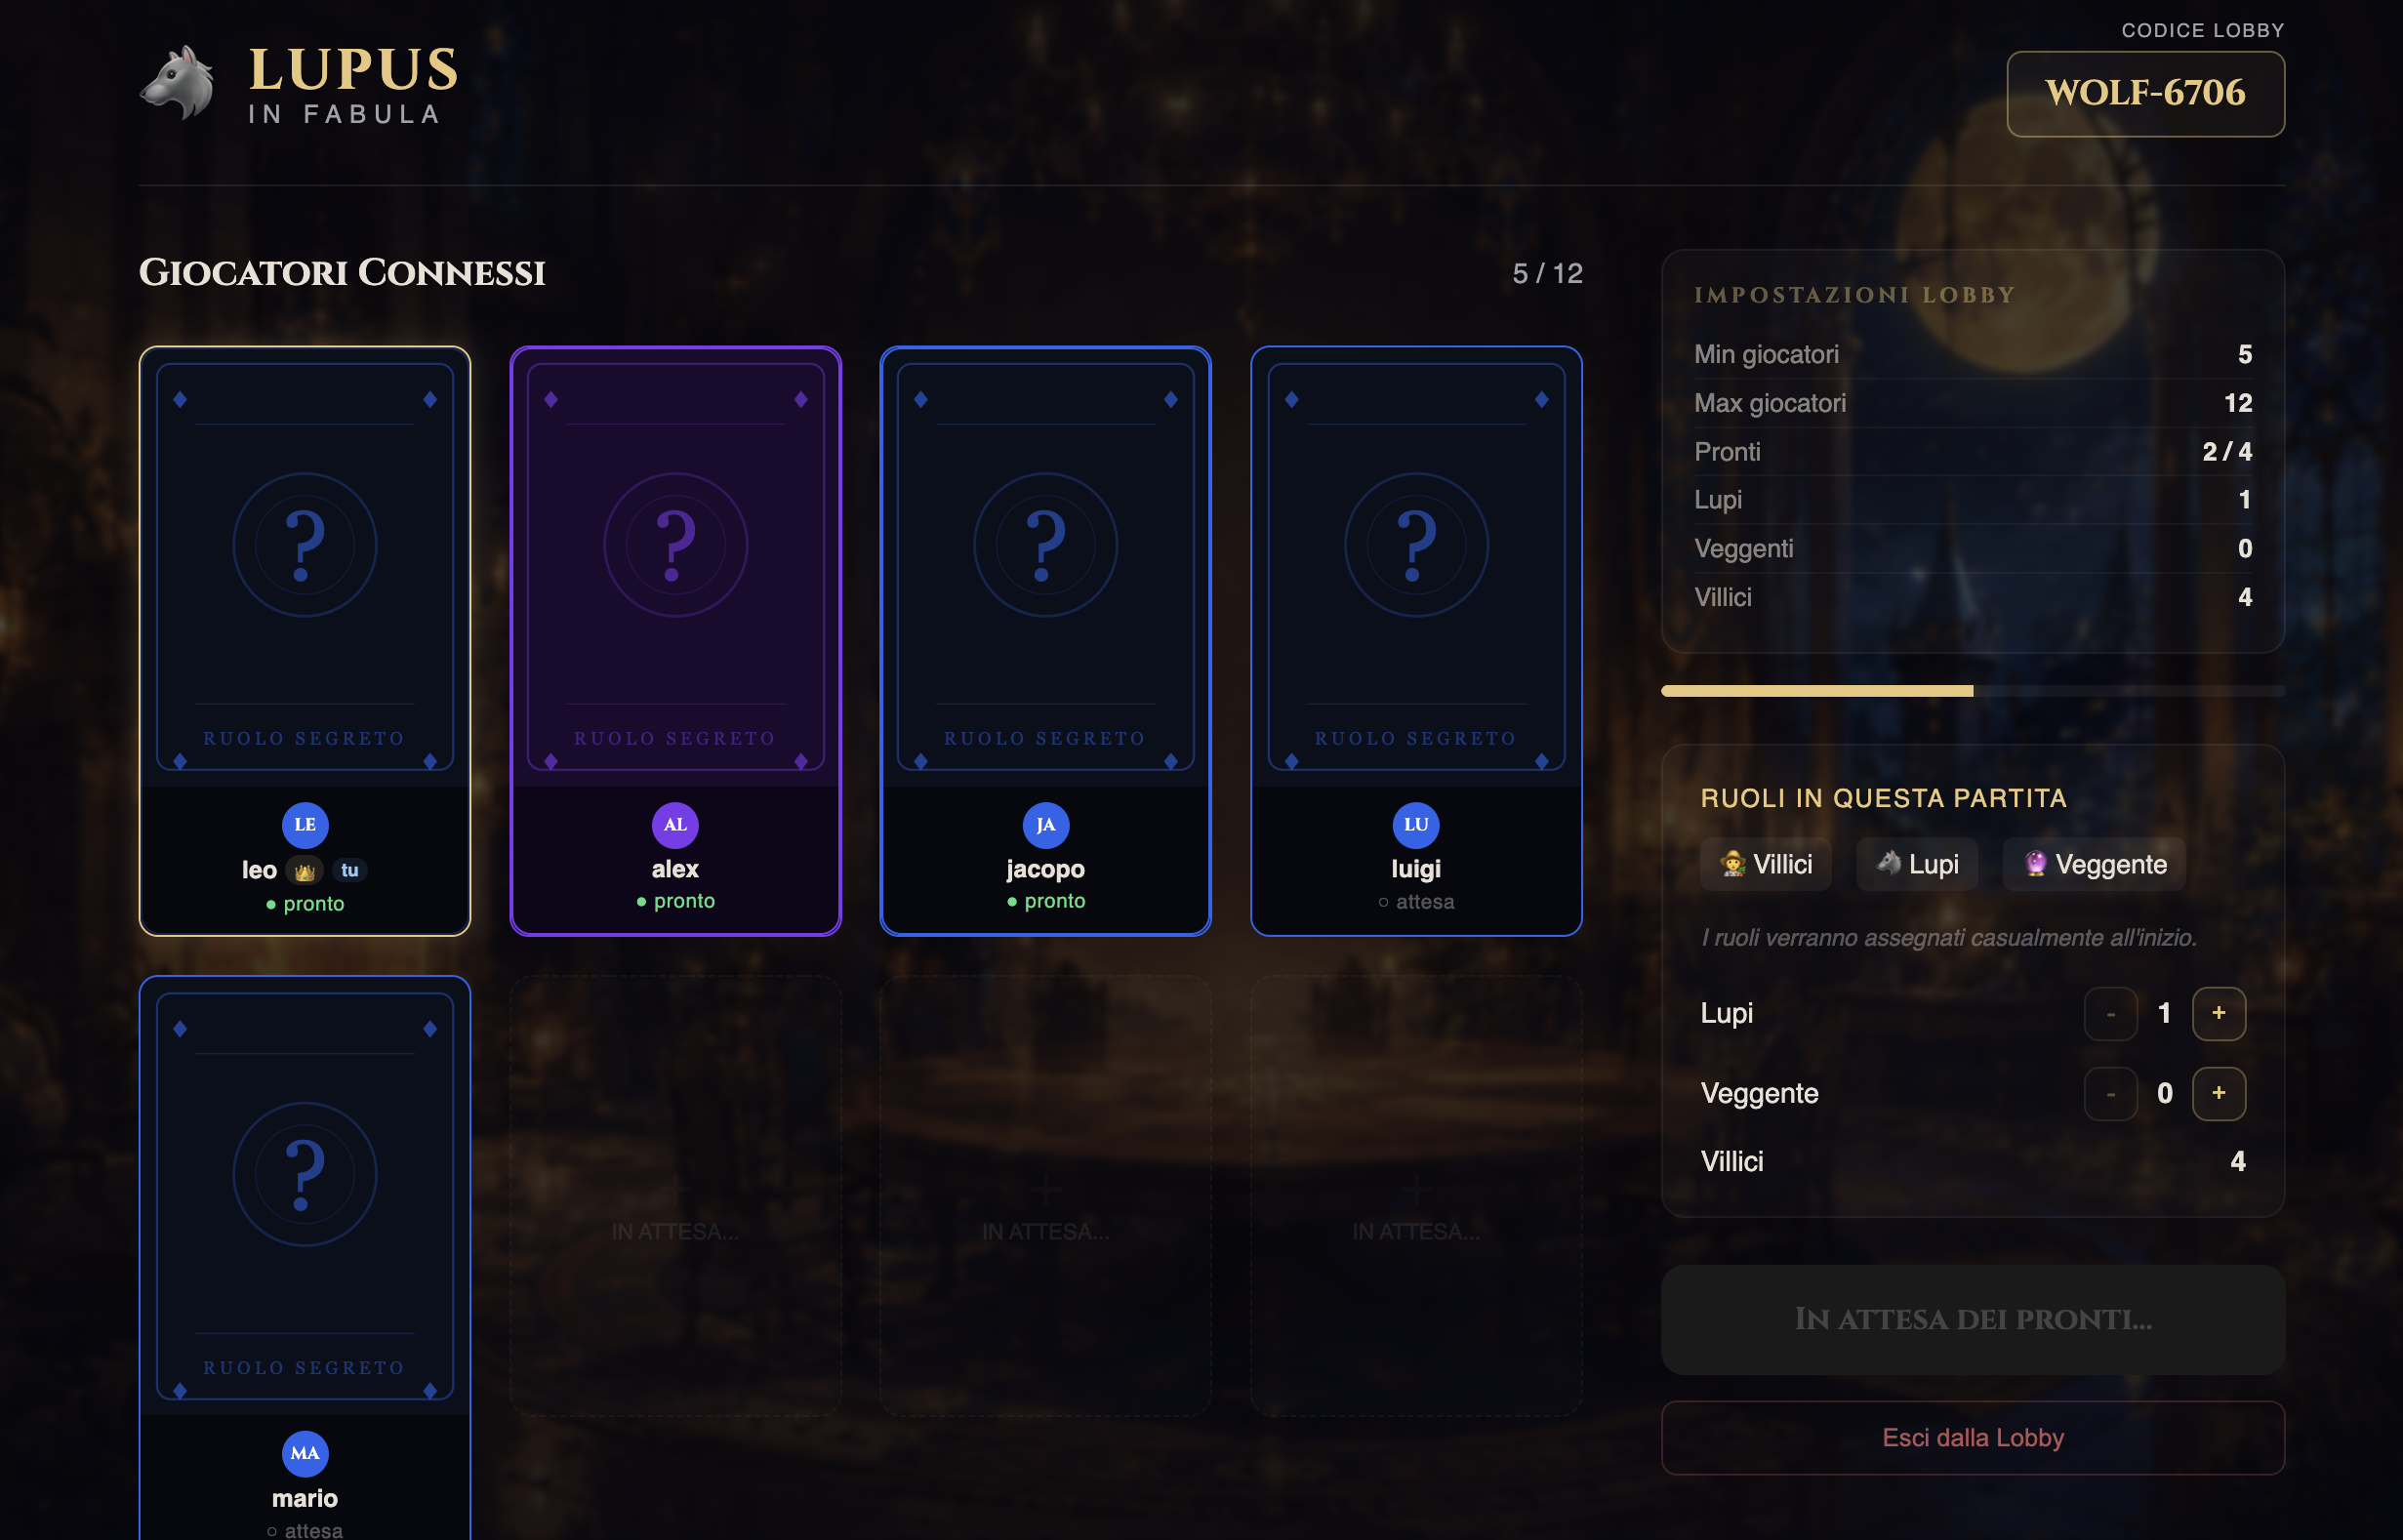
\includegraphics[width=0.8\textwidth]{figures/screenshot_lobby.png}
      \caption{Lobby screen: room code, connected players and their \emph{Ready}
            status, and the game-configuration panel.}
      \label{fig:screenshot-lobby}
\end{figure}

\begin{figure}
      \centering
      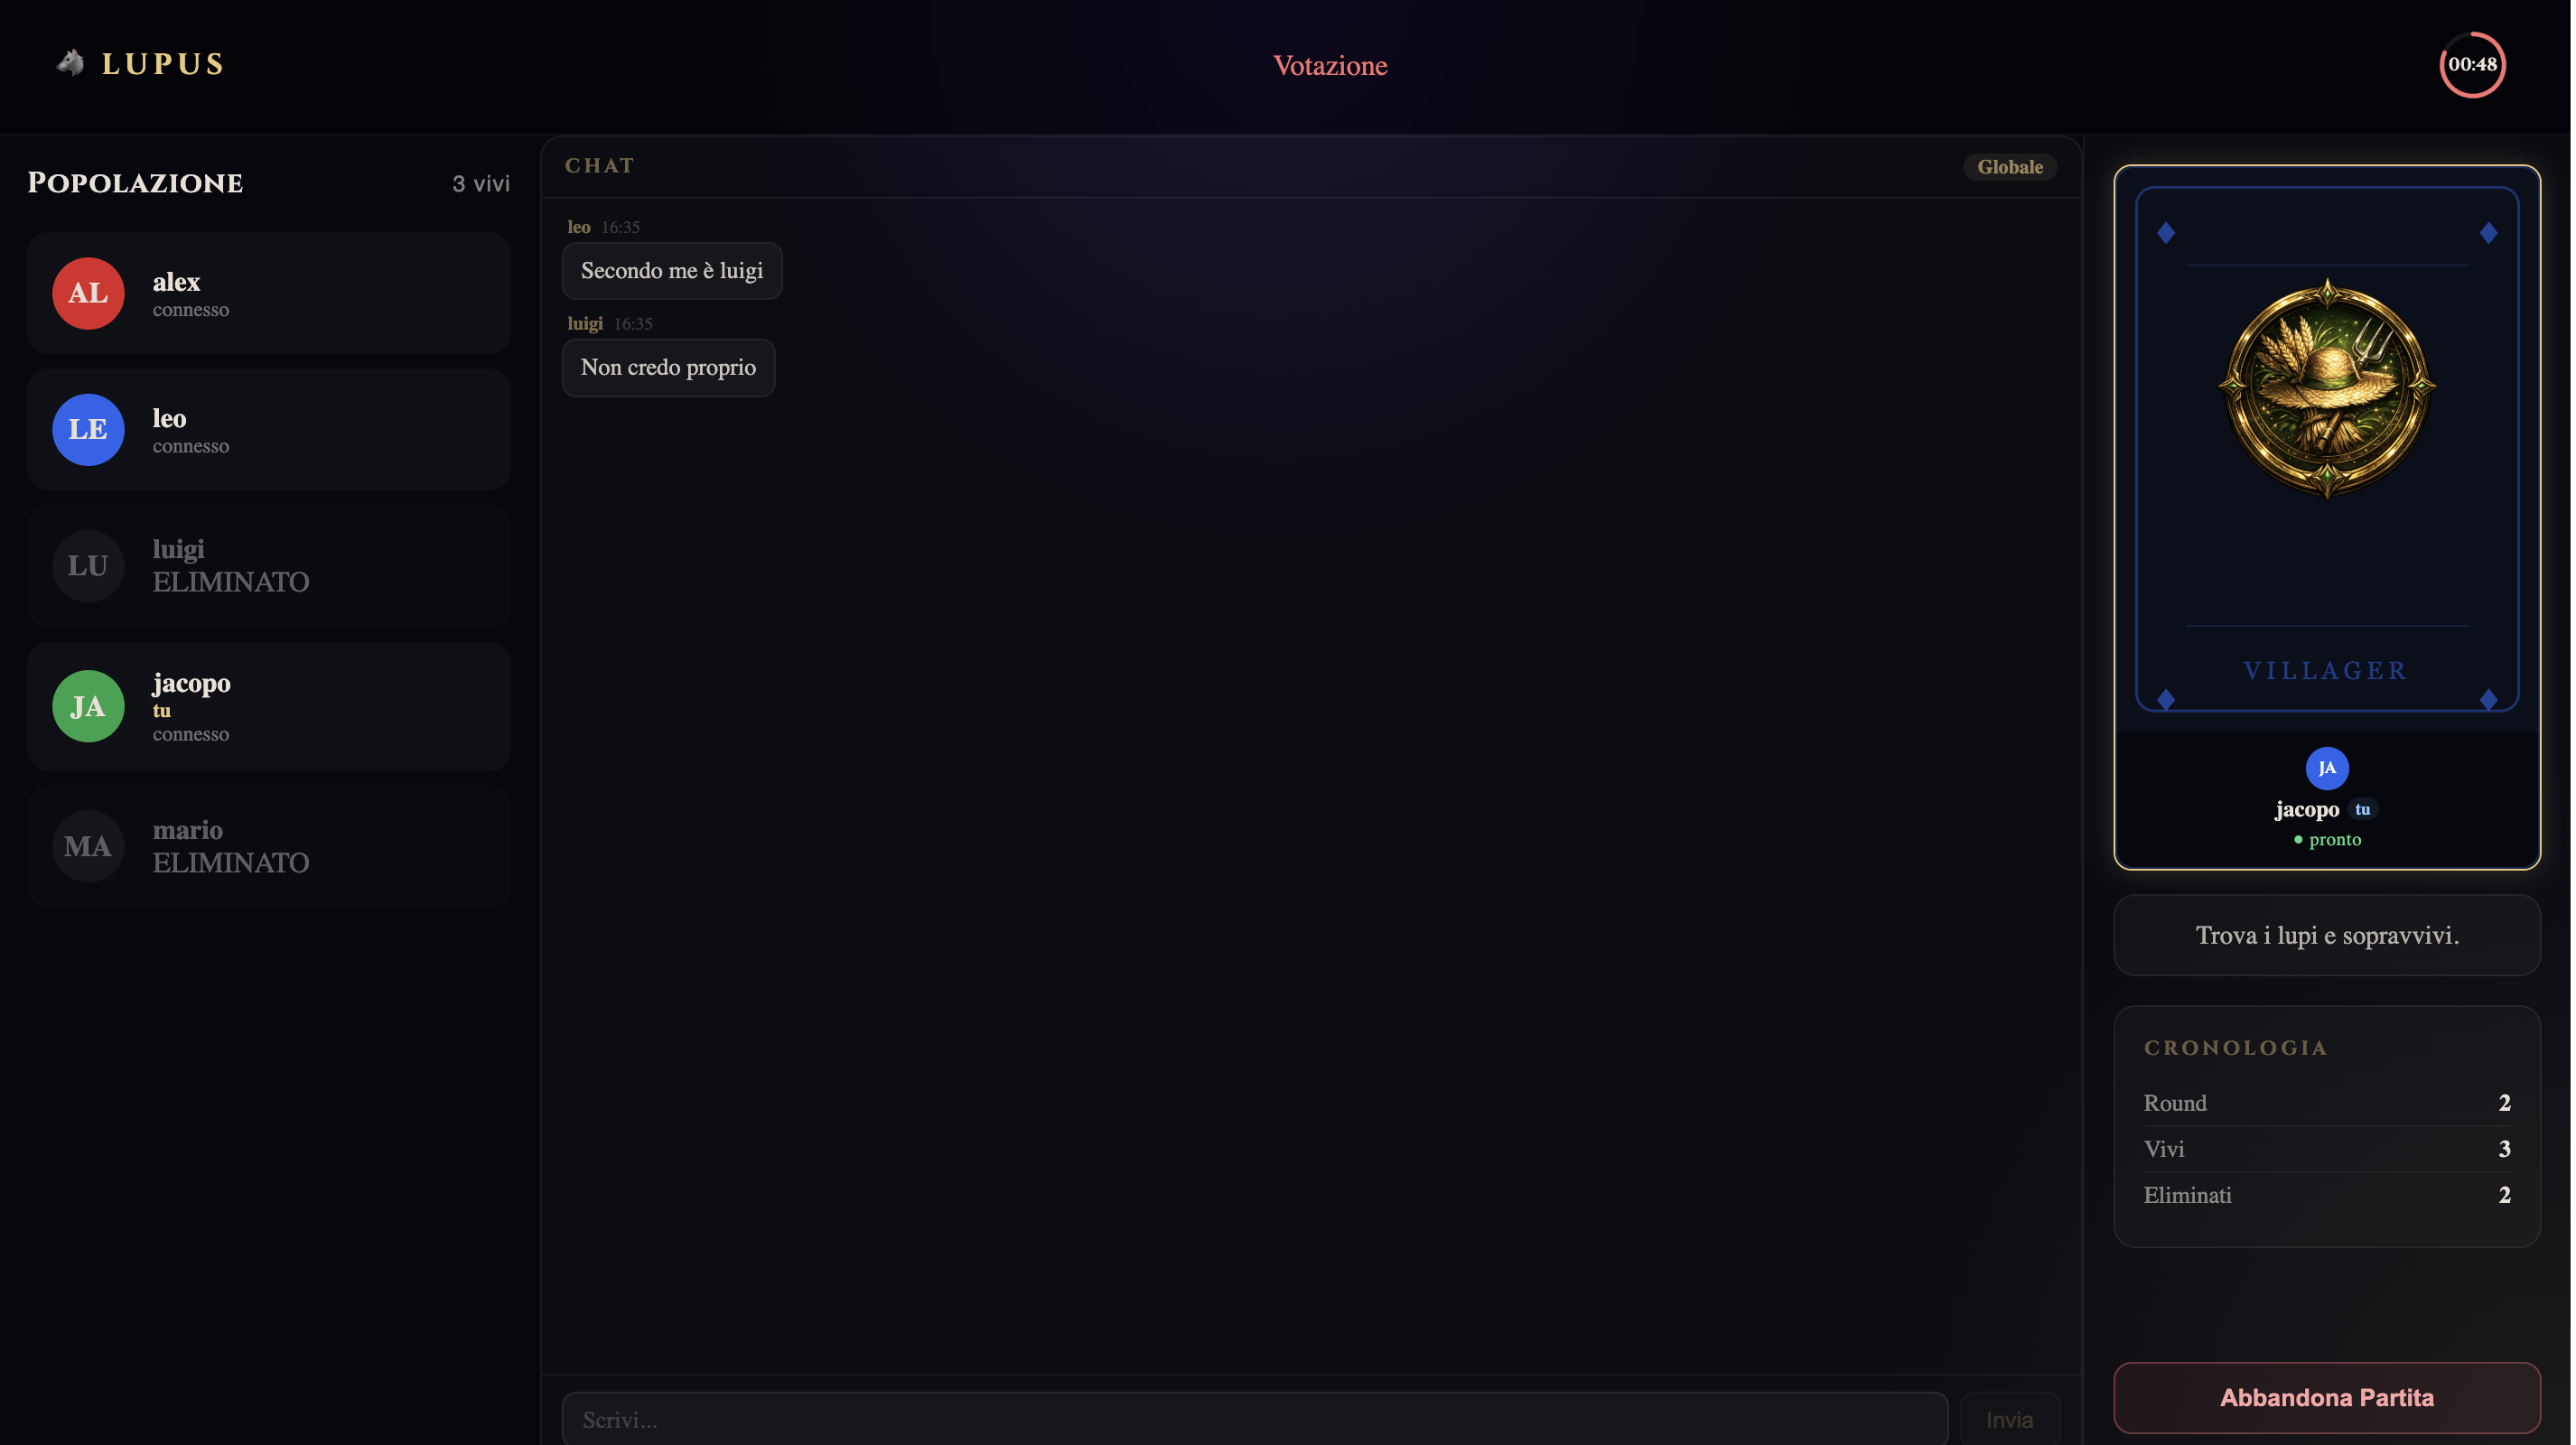
\includegraphics[width=0.8\textwidth]{figures/screenshot_game_day.png}
      \caption{Game screen during the day phase, while voting is in progress.}
      \label{fig:screenshot-game-day}
\end{figure}

\begin{figure}
      \centering
      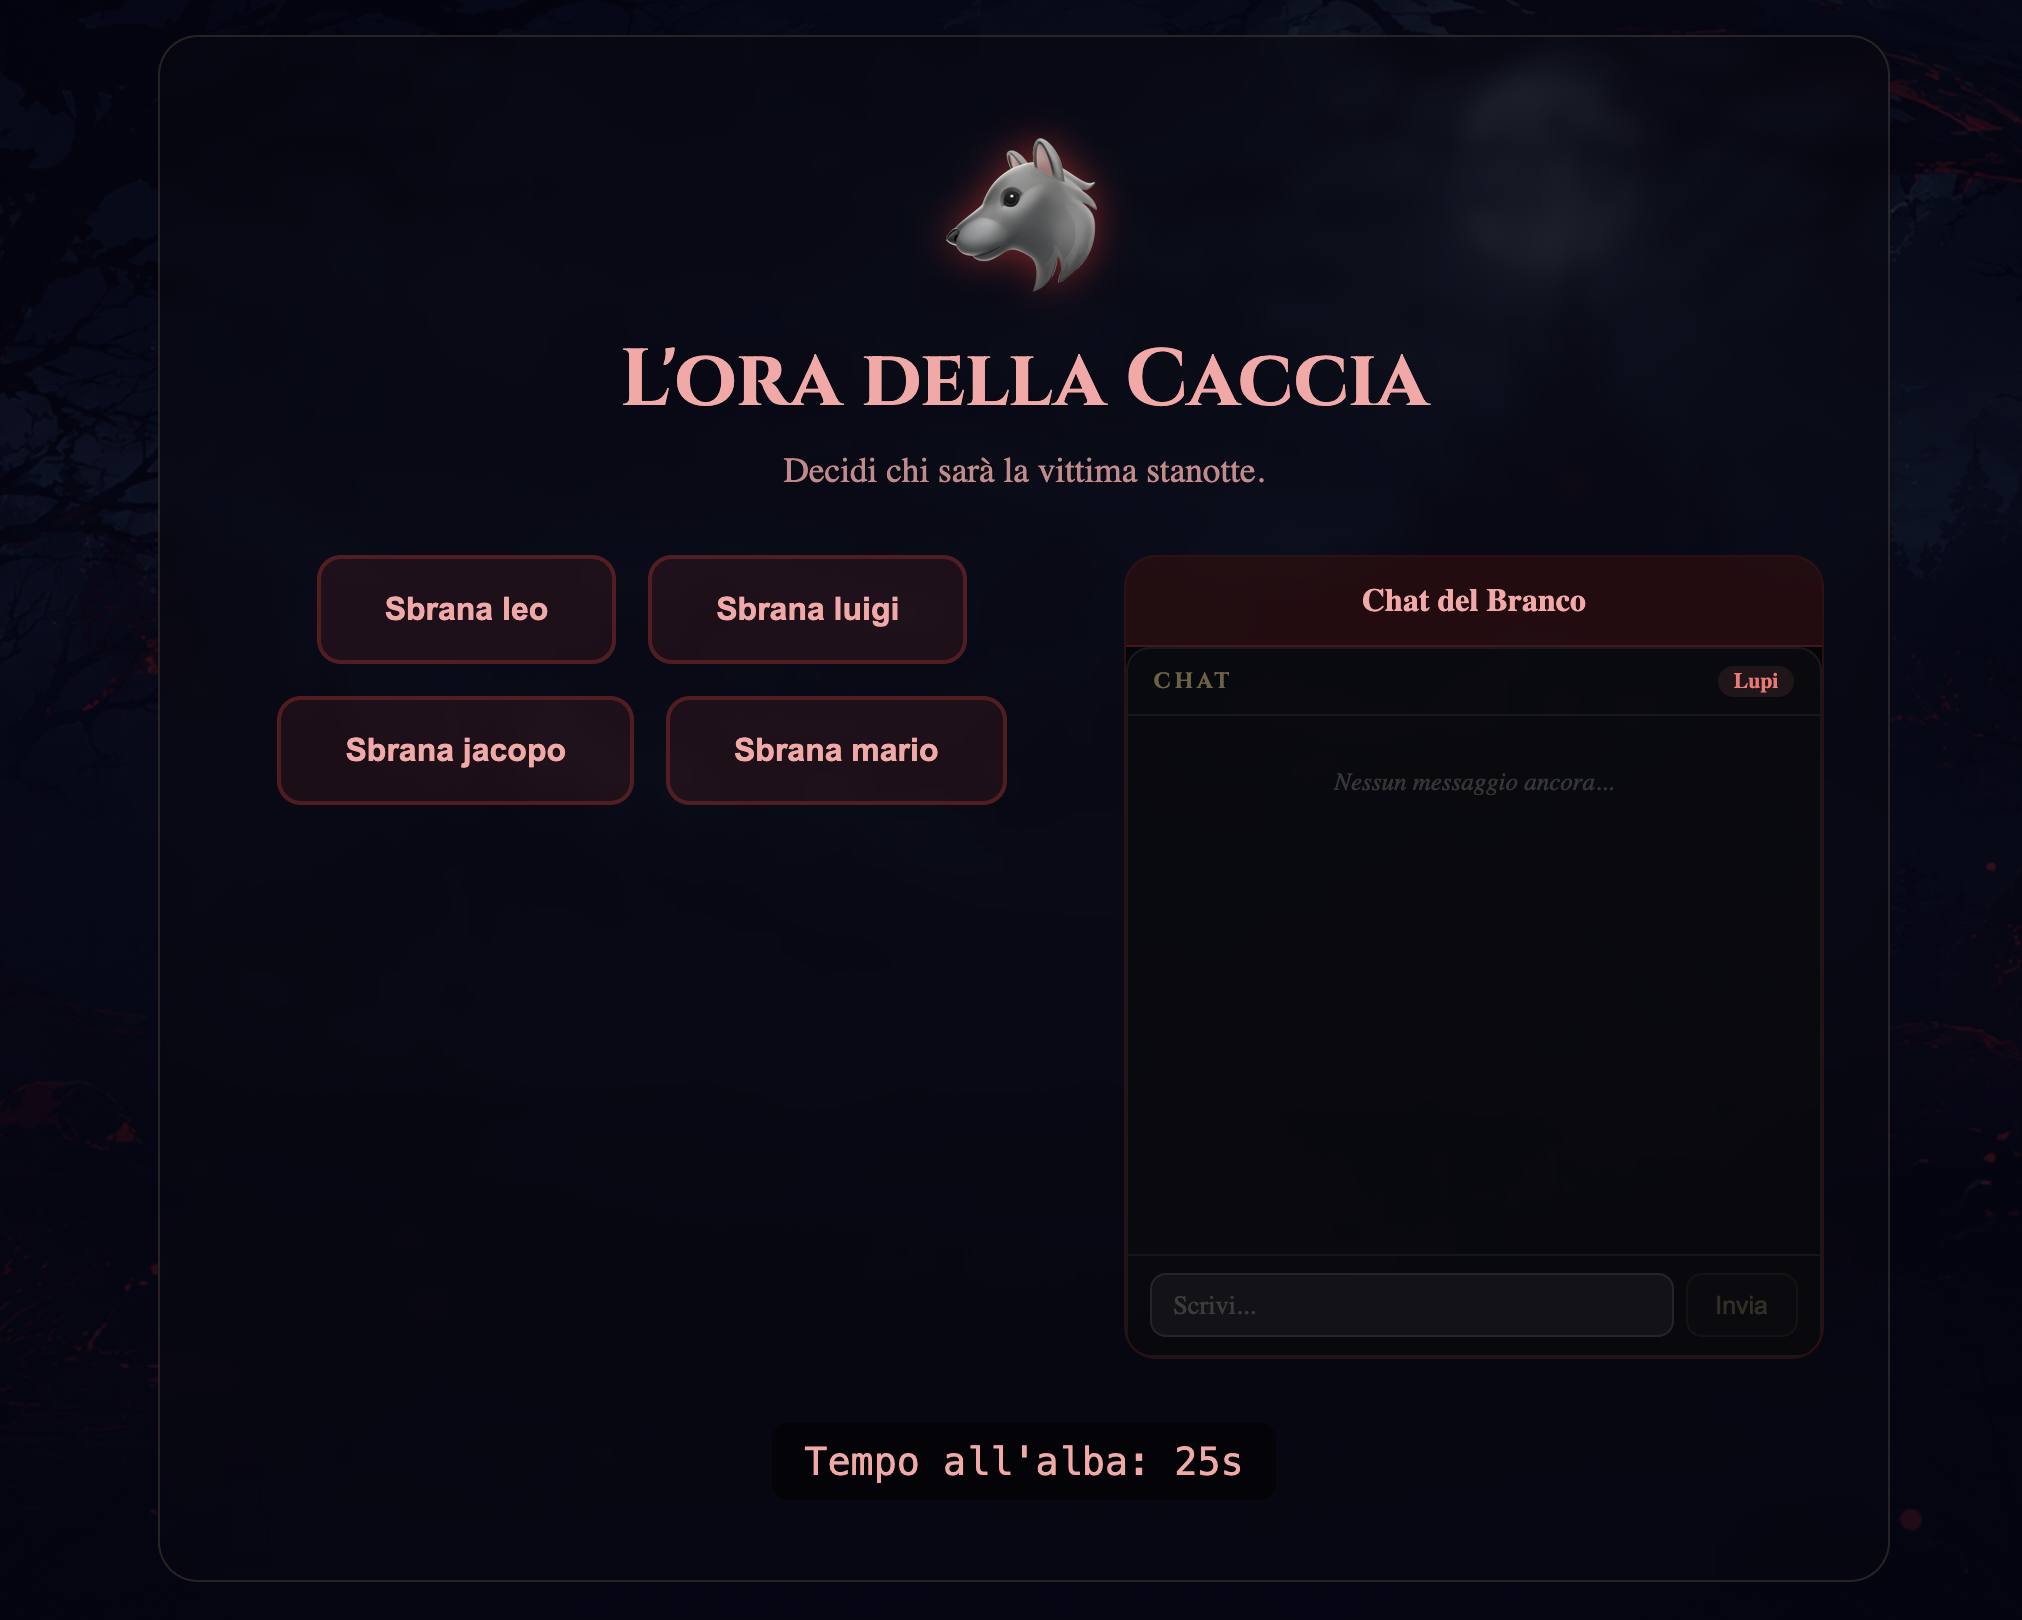
\includegraphics[width=0.8\textwidth]{figures/screenshot_game_night.png}
      \caption{Game screen during the night phase, showing the actions available only
            to the wolves and the seer.}
      \label{fig:screenshot-game-night}
\end{figure}

\begin{figure}
      \centering
      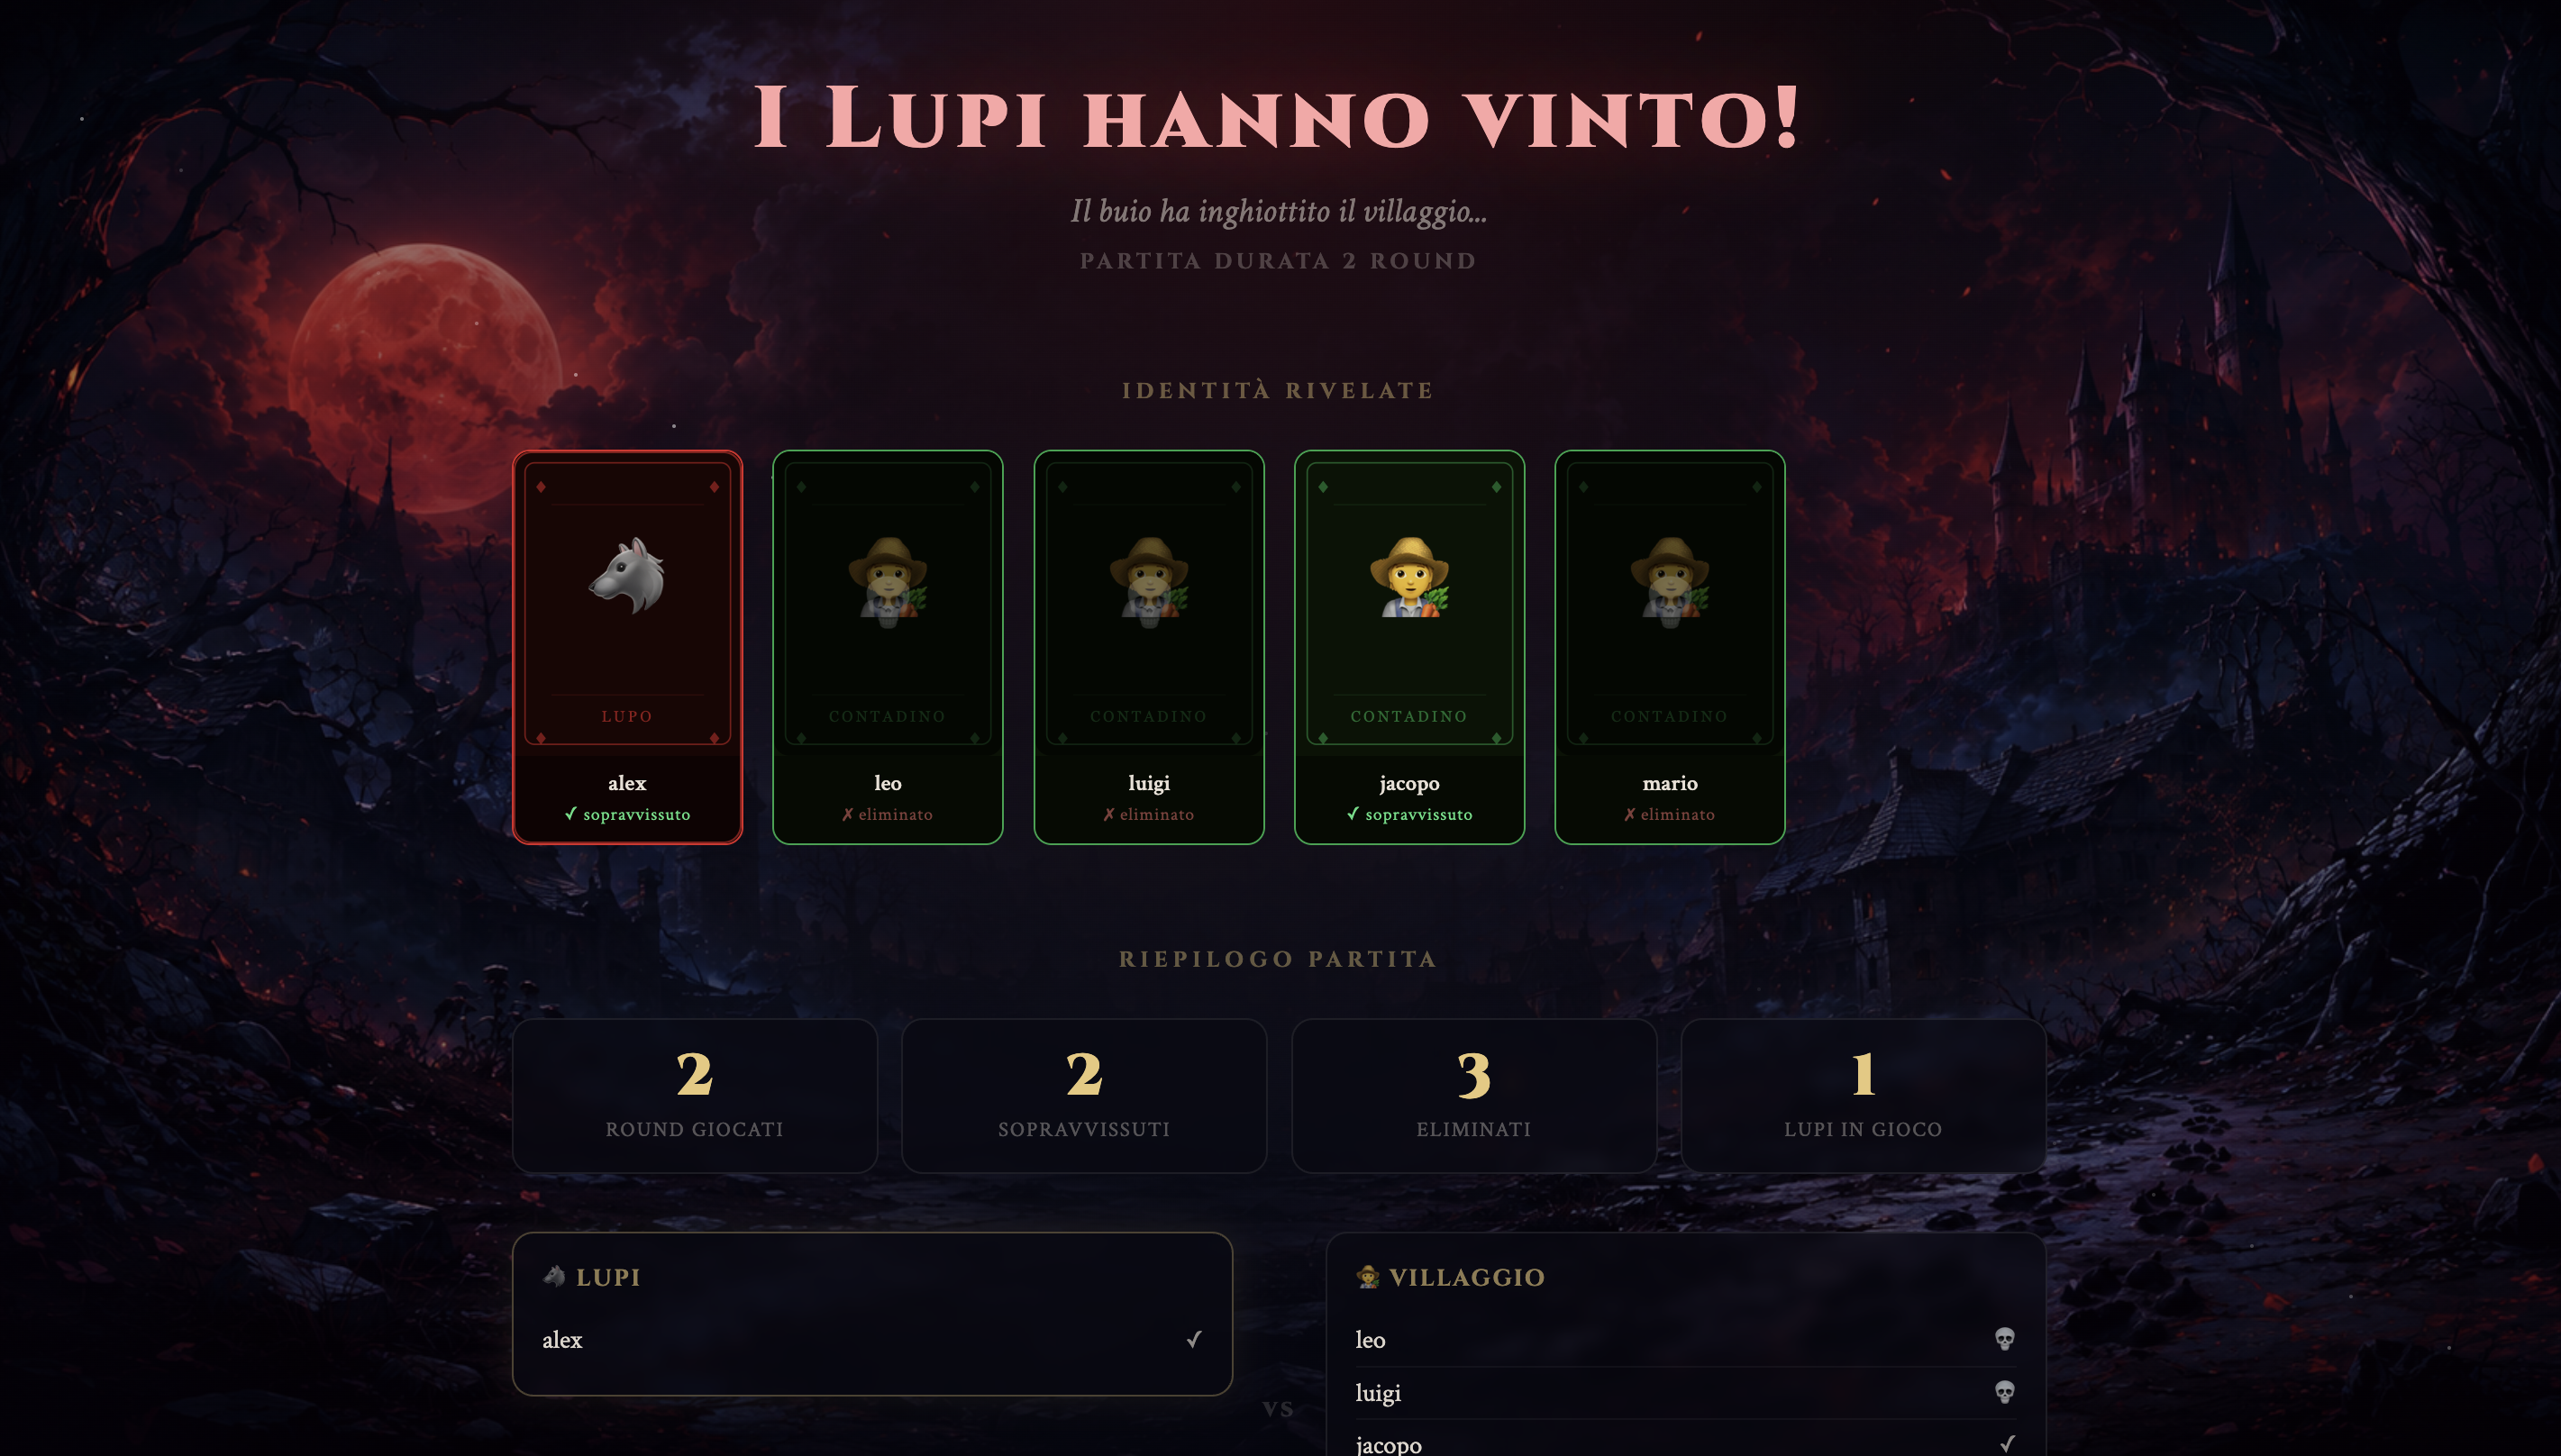
\includegraphics[width=0.8\textwidth]{figures/screenshot_results.png}
      \caption{Final results screen announcing the winning team and revealing all
            player roles.}
      \label{fig:screenshot-results}
\end{figure}

\section{Self-evaluation}\label{self-evaluation}

Each member is responsible only for their own subsection.

\subsection{Jacopo Bonifazi --- Frontend \& Lobby}

My role in the group was to design and implement the entire frontend and the
lobby system: the user interface (home, lobby, game, and results screens), the
client-side state management with three Pinia stores, the integration with the
real-time channel via the Socket.IO client, and the client-side handling of
disconnection and recovery. I also owned the definition of the Socket.IO event
contract on the client side, in coordination with the backend.

\paragraph{Strengths of the product.} The client is cleanly layered and
event-driven, which keeps game logic entirely on the server and makes the UI a
pure projection of the authoritative state; this made the resynchronisation after
a fault straightforward and robust. The restricted-visibility chat and the
per-role, per-phase action gating meet the functional requirements, and the
message de-duplication correctly handles the at-least-once delivery that arises in
the multi-instance deployment.

\paragraph{Weaknesses / limitations.} The pause/resume experience depends on
server-side events that were still being finalised, so its full behaviour was not
completely exercised. The component-level UI is validated mostly by manual
end-to-end testing rather than automated component tests. Some auxiliary REST
scaffolding remained unused once the interaction consolidated on the event
channel.

\paragraph{Contribution.} Objectively, I delivered the full frontend and lobby as
planned, and additionally helped diagnose several integration issues that surfaced
in the containerised, multi-instance environment (e.g.\ the WebSocket endpoint
mismatch and the instance-local player counting), which, although resolved
server-side/infrastructure-side, were identified from the client behaviour.

\subsection{Alexandru Nicolescu --- Infrastructure \& Distribution}

My role in the group was the \emph{distribution and infrastructure} side of the
project: I designed and built the deployment layer (the Docker images and Compose
topology with its segregated networks and health checks, the NGINX reverse-proxy
configuration for WebSocket balancing, the full set of Kubernetes manifests with
HPA and rolling updates, and the Prometheus/Grafana monitoring stack), I led the
migration of the realtime layer from raw WebSocket to Socket.IO, and I implemented
the cross-replica machinery: the Redis Pub/Sub manager with sender-based
deduplication, retries and reconnection, and the distributed-safety mechanisms
(atomic host election, phase-advancement lock, optimistic state patches, timer
sweeper, anti-entropy). I also wrote the infrastructure-level validation: the
multi-instance, reconnection, and distributed-safety suites, and the multi-process
load generator.

The main strength of this part of the product, in my view, is that replication is
real and tested, not nominal: the platform genuinely survives replica kills
mid-match, and every claimed guarantee has a test that encodes its race condition.
I am also satisfied with the symmetry between the Compose and Kubernetes
environments, which made every production-like experiment cheap.

The main weaknesses I recognise are, first, that Redis remains a single stateful
point of failure --- mitigated by persistence and by how the rest of the system
degrades, but not eliminated (an HA store was beyond the time budget, see
\cref{future-works}); and second, that some convergence guarantees rest on
periodic anti-entropy rather than on acknowledged delivery, which is adequate for
a game but required care to reason about and would not transfer as-is to a domain
with stricter requirements. Working through those trade-offs --- and discovering
how many ``obvious'' single-node behaviours (timers, session counting, private
messages) silently break under replication --- was the most instructive part of
the course project for me.

\subsection{Leonardo Vorabbi --- Backend}

Within the group, I was responsible for the backend of the project, focusing on
the server-side logic of the application. My main responsibilities included
designing and implementing the backend architecture, managing game and lobby
state, implementing the Redis-based persistence layer, handling Socket.IO events
and real-time server--client communication, managing phase transitions and
timers, defining the game logic and validation rules for actions, voting, and
role-based behavior, and implementing and maintaining the backend test suite.

From my point of view, the main strengths of the product lie in its
stateless-at-process-level backend architecture, which makes horizontal scaling
practical, and in the hybrid communication model, combining REST for simple
queries with Socket.IO/WebSocket for real-time gameplay. The system supports
multiple backend replicas and keeps working correctly even when players are
connected to different instances. The codebase is organized into clearly separated
layers (models, state management, game logic, transport), and is backed by a test
suite covering unit tests, integration tests, distributed-safety checks, and
end-to-end scenarios.

The main weaknesses concern authentication, which is intentionally lightweight and
based on client-side session identifiers, and could therefore be unsuitable for a
production environment requiring strong identity management.

\section{Future works}\label{future-works}

The current implementation already provides a complete distributed real-time game
platform, but several directions remain open to strengthen robustness, simplify
maintenance, and extend gameplay.

\begin{description}
      \item[High-availability store.] The single Redis instance is the one component
            whose failure pauses the whole platform (\cref{fault-tolerance}). The natural
            evolution is Redis Sentinel (primary/replica with automatic failover) --- the
            client library already supports it, so the change is confined to configuration
            and manifests --- or, at larger scale, Redis Cluster with per-room key hashtags
            so that each room's keys stay on one shard and the existing transactions keep
            working.

      \item[Strong authentication and persistent identities.] Client identity is
            currently a lightweight value in \texttt{sessionStorage} passed in the Socket.IO
            handshake. A production-grade solution would introduce a JWT/OAuth login flow,
            require the signed token on both REST and Socket.IO connections, and persist
            user profiles (username, avatar, match history) in a database, making host
            privileges and player identity independent of client-provided values.

      \item[At-least-once event delivery.] Convergence currently relies on periodic
            anti-entropy over an at-most-once bus. Replacing room channels with \emph{Redis
                  Streams} and consumer groups would give persistent, acknowledged, replayable
            per-room event logs --- turning reconnection into a replay from the last seen
            event id and making the snapshot re-broadcast a rare repair path instead of a
            periodic one.

      \item[Connection-aware autoscaling.] The HPA currently scales on CPU/memory,
            which under-represents a connection-bound workload (\cref{availability}). The
            backend already exports an active-connections metric per replica, and the
            manifest documents the Pods-metric block to scale on it; enabling it only
            requires installing the Prometheus Adapter in the cluster.

      \item[Persistence of chat and match history.] Chat messages currently live only
            in the real-time channel, with no long-term history. Storing them in a database
            or a per-room Redis list, adding pagination, and persisting match summaries
            (phases, eliminations, winners) would enable a history/replay page and improve
            debuggability.

      \item[Richer matchmaking and lobby management.] The lobby workflow could be
            extended with public/private rooms and filters, automatic room assignment,
            invite links or QR codes, and room templates for different rule sets.

      \item[More roles and configurable rule variants.] The fixed core role set and
            phase structure could gain roles such as Hunter, Doctor, or Cupid, with role
            composition and game mode externalised into a configuration file selectable by
            the host before the match. The event-based design keeps this cheap: a new role
            is a new payload type, new validation rules, and new private events, with no
            change to the distribution machinery.

      \item[Frontend polish.] Complete the pause/resume UX once the corresponding
            server events are finalised (including a graceful ``player did not return''
            outcome), add automated component/end-to-end tests to cover the UI flows
            currently checked manually, remove the unused REST scaffolding now that
            interaction is event-based, and add richer, always-legible error feedback on the
            entry screen.

      \item[Security hardening and operational polish.] TLS termination at the
            proxy/Ingress (ports and headers are already prepared), Redis authentication
            (the Secret template exists), stricter CORS and WebSocket origin checks, rate
            limiting on sensitive actions, and protected monitoring endpoints; plus a CI
            pipeline running the three test rings on every push, image publication to a
            registry with digest pinning, and structured JSON logging shipped to a log
            aggregator to complement metrics.
\end{description}

\bibliographystyle{plain}
\bibliography{references}

\end{document}
